\documentclass{book}
\usepackage{fontspec}
\setmainfont{STIX Two Text}

%PACKAGES
\iffalse
Here are the packages that I use
\fi

\usepackage{blindtext, hyperref, verbatim, minted, graphicx, amssymb, textcomp, enumerate, tcolorbox, newunicodechar, textgreek, wasysym, tipa, eso-pic, lipsum, bbold, dsfont}
\usepackage[margin=1.3in]{geometry}
\usepackage{longtable}
\usepackage{newunicodechar}
\usepackage{amsthm}
\usepackage{tikz}
\usepackage{tikz-cd}




%ENVIRONMENTS

%Here I define some common environments. I use definitions, theorems, examples, and lemmas.


\theoremstyle{definition}
\newtheorem{definition}{Definition}
\newtheorem{theorem}{Theorem}
\newtheorem{example}{Example}
\newtheorem{lemma}{Lemma}


\newunicodechar{ₙ}{${}_{n}$}

\newunicodechar{𝓓}{$\mathcal{D}$}
\newunicodechar{∂}{$\partial$}
\newunicodechar{∇}{\raisebox{-0.05cm}{$\nabla$}}

%\newunicodechar{Π⃗}{$\stackrel{\arr}{\pi}$}

\newunicodechar{×}{$\times$}
\newunicodechar{→}{$\rightarrow$}
\newunicodechar{⟨}{$\langle$}
\newunicodechar{⟩}{$\rangle$}
\newunicodechar{↦}{$\mapsto$}
\newunicodechar{∧}{$\wedge$}
\newunicodechar{∨}{$\vee$}
\newunicodechar{∃}{$\exists$}
\newunicodechar{∀}{$\forall$}
\newunicodechar{¬}{$\neg$}
\newunicodechar{ᵃ}{${}^{\texttt{a}}$}
\newunicodechar{ᵇ}{${}^{\texttt{b}}$}
\newunicodechar{ᶜ}{${}^{\texttt{c}}$}
\newunicodechar{ᵈ}{${}^{\texttt{d}}$}
\newunicodechar{ᵉ}{${}^{\texttt{e}}$}
\newunicodechar{ᶠ}{${}^{\texttt{f}}$}
\newunicodechar{ᵍ}{${}^{\texttt{g}}$}
\newunicodechar{ʰ}{${}^{\texttt{h}}$}
\newunicodechar{ⁱ}{${}^{\texttt{i}}$}
\newunicodechar{ʲ}{${}^{\texttt{j}}$}
\newunicodechar{ᵏ}{${}^{\texttt{k}}$}
\newunicodechar{ˡ}{${}^{\texttt{l}}$}
\newunicodechar{ᵐ}{${}^{\texttt{m}}$}
\newunicodechar{ⁿ}{${}^{\texttt{n}}$}
\newunicodechar{ᵒ}{${}^{\texttt{o}}$}
\newunicodechar{ᵖ}{${}^{\texttt{p}}$}
\newunicodechar{ʳ}{${}^{\texttt{r}}$}
\newunicodechar{ˢ}{${}^{\texttt{s}}$}
\newunicodechar{ᵗ}{${}^{\texttt{t}}$}
\newunicodechar{ᵘ}{${}^{\texttt{u}}$}
\newunicodechar{ᵛ}{${}^{\texttt{v}}$}
\newunicodechar{ʷ}{${}^{\texttt{w}}$}
\newunicodechar{ˣ}{${}^{\texttt{x}}$}
\newunicodechar{ʸ}{${}^{\texttt{y}}$}
\newunicodechar{ᶻ}{${}^{\texttt{z}}$}
\newunicodechar{⁰}{${}^{\texttt{0}}$}
\newunicodechar{¹}{${}^{\texttt{1}}$}
\newunicodechar{²}{${}^{\texttt{2}}$}
\newunicodechar{³}{${}^{\texttt{3}}$}
\newunicodechar{⁴}{${}^{\texttt{4}}$}
\newunicodechar{⁵}{${}^{\texttt{5}}$}
\newunicodechar{⁶}{${}^{\texttt{6}}$}
\newunicodechar{⁷}{${}^{\texttt{7}}$}
\newunicodechar{⁸}{${}^{\texttt{8}}$}
\newunicodechar{⁹}{${}^{\texttt{9}}$}
\newunicodechar{⁻}{${}^{\texttt{-}}$}
\newunicodechar{ᵒ}{${}^{\texttt{o}}$}
\newunicodechar{ᵖ}{${}^{\texttt{ω}}$}
\newunicodechar{⁻}{${}^{\texttt{-}}$}
\newunicodechar{¹}{${}^{\texttt{1}}$}
\newunicodechar{₀}{${}_{\texttt{0}}$}
\newunicodechar{₁}{${}_{\texttt{1}}$}
\newunicodechar{₂}{${}_{\texttt{2}}$}
\newunicodechar{₃}{${}_{\texttt{3}}$}
\newunicodechar{₄}{${}_{\texttt{4}}$}
\newunicodechar{₅}{${}_{\texttt{5}}$}
\newunicodechar{₆}{${}_{\texttt{6}}$}
\newunicodechar{₇}{${}_{\texttt{7}}$}
\newunicodechar{₈}{${}_{\texttt{8}}$}
\newunicodechar{₉}{${}_{\texttt{9}}$}

\newunicodechar{𝔸}{$\mathbb{A}$}
\newunicodechar{𝔹}{$\mathbb{B}$}
\newunicodechar{ℂ}{$\mathbb{C}$}
\newunicodechar{𝔻}{$\mathbb{D}$}
\newunicodechar{𝔼}{$\mathbb{E}$}
\newunicodechar{𝔽}{$\mathbb{F}$}
\newunicodechar{𝔾}{$\mathbb{G}$}
\newunicodechar{ℍ}{$\mathbb{H}$}
\newunicodechar{𝕀}{$\mathbb{I}$}
\newunicodechar{𝕁}{$\mathbb{J}$}
\newunicodechar{𝕂}{$\mathbb{K}$}
\newunicodechar{𝕃}{$\mathbb{L}$}
\newunicodechar{𝕄}{$\mathbb{M}$}
\newunicodechar{ℕ}{$\mathbb{N}$}
\newunicodechar{𝕆}{$\mathbb{O}$}
\newunicodechar{ℙ}{$\mathbb{P}$}
\newunicodechar{ℚ}{$\mathbb{Q}$}
\newunicodechar{ℝ}{$\mathbb{R}$}
\newunicodechar{𝕊}{$\mathbb{S}$}
\newunicodechar{𝕋}{$\mathbb{T}$}
\newunicodechar{𝕌}{$\mathbb{U}$}
\newunicodechar{𝕍}{$\mathbb{V}$}
\newunicodechar{𝕎}{$\mathbb{W}$}
\newunicodechar{𝕏}{$\mathbb{X}$}
\newunicodechar{𝕐}{$\mathbb{Y}$}
\newunicodechar{ℤ}{$\mathbb{Z}$}

\newunicodechar{𝚫}{$\Delta$}
\newunicodechar{ʃ}{$\int$}
\newunicodechar{∪}{$\cup$}
\newunicodechar{∩}{$\cap$}
\newunicodechar{±}{$\pm$}
\newunicodechar{𝔄}{$\mathfrak{A}$}




\newunicodechar{𝔅}{$\mathfrak{B}$}
\newunicodechar{ℭ}{$\mathfrak{C}$}
\newunicodechar{𝔇}{$\mathfrak{D}$}
\newunicodechar{𝔈}{$\mathfrak{E}$}
\newunicodechar{𝔉}{$\mathfrak{F}$}
\newunicodechar{𝔊}{$\mathfrak{G}$}
\newunicodechar{ℌ}{$\mathfrak{H}$}
\newunicodechar{ℑ}{$\mathfrak{I}$}
\newunicodechar{𝔍}{$\mathfrak{J}$}
\newunicodechar{𝔎}{$\mathfrak{K}$}
\newunicodechar{𝔏}{$\mathfrak{L}$}
\newunicodechar{𝔐}{$\mathfrak{M}$}
\newunicodechar{𝔑}{$\mathfrak{N}$}
\newunicodechar{𝔒}{$\mathfrak{O}$}
\newunicodechar{𝔓}{$\mathfrak{P}$}
\newunicodechar{𝔔}{$\mathfrak{Q}$}
\newunicodechar{ℜ}{$\mathfrak{R}$}
\newunicodechar{𝔖}{$\mathfrak{S}$}
\newunicodechar{𝔗}{$\mathfrak{T}$}
\newunicodechar{𝔘}{$\mathfrak{U}$}
\newunicodechar{𝔙}{$\mathfrak{V}$}
\newunicodechar{𝔚}{$\mathfrak{W}$}
\newunicodechar{𝔛}{$\mathfrak{X}$}
\newunicodechar{𝔜}{$\mathfrak{Y}$}
\newunicodechar{ℨ}{$\mathfrak{Z}$}

\newunicodechar{𝔞}{$\mathfrak{a}$}
\newunicodechar{𝔟}{$\mathfrak b$}
\newunicodechar{𝔠}{$\mathfrak{c}$}
\newunicodechar{𝔡}{$\mathfrak{d}$}
\newunicodechar{𝔢}{$\mathfrak{e}$}
\newunicodechar{𝔣}{$\mathfrak{f}$}
\newunicodechar{𝔤}{$\mathfrak{g}$}
\newunicodechar{𝔥}{$\mathfrak{h}$}
\newunicodechar{𝔦}{$\mathfrak{i}$}
\newunicodechar{𝔧}{$\mathfrak{j}$}
\newunicodechar{𝔨}{$\mathfrak{k}$}
\newunicodechar{𝔩}{$\mathfrak{l}$}
\newunicodechar{𝔪}{$\mathfrak{m}$}
\newunicodechar{𝔫}{$\mathfrak{n}$}
\newunicodechar{𝔬}{$\mathfrak{o}$}
\newunicodechar{𝔭}{$\mathfrak{ω}$}
\newunicodechar{𝔮}{$\mathfrak{q}$}
\newunicodechar{𝔯}{$\mathfrak{r}$}
\newunicodechar{𝔰}{$\mathfrak{s}$}
\newunicodechar{𝔱}{$\mathfrak{t}$}
\newunicodechar{𝔲}{$\mathfrak{u}$}
\newunicodechar{𝔳}{$\mathfrak{v}$}
\newunicodechar{𝔴}{$\mathfrak{w}$}
\newunicodechar{𝔵}{$\mathfrak{x}$}
\newunicodechar{𝔶}{$\mathfrak{y}$}
\newunicodechar{𝔷}{$\mathfrak{z}$}

\newunicodechar{𝐀}{${\bf{A}}$}
\newunicodechar{𝐁}{${\bf{B}}$}
\newunicodechar{𝐂}{${\bf{C}}$}
\newunicodechar{𝐃}{${\bf{D}}$}
\newunicodechar{𝐄}{${\bf{E}}$}
\newunicodechar{𝐅}{${\bf{F}}$}
\newunicodechar{𝐆}{${\bf{G}}$}
\newunicodechar{𝐇}{${\bf{H}}$}
\newunicodechar{𝐈}{${\bf{I}}$}
\newunicodechar{𝐉}{${\bf{J}}$}
\newunicodechar{𝐊}{${\bf{K}}$}
\newunicodechar{𝐋}{${\bf{L}}$}
\newunicodechar{𝐌}{${\bf{M}}$}
\newunicodechar{𝐍}{${\bf{N}}$}
\newunicodechar{𝐎}{${\bf{O}}$}
\newunicodechar{𝐏}{${\bf{P}}$}
\newunicodechar{𝐐}{${\bf{Q}}$}
\newunicodechar{𝐑}{${\bf{R}}$}
\newunicodechar{𝐒}{${\bf{S}}$}
\newunicodechar{𝐓}{${\bf{T}}$}
\newunicodechar{𝐔}{${\bf{U}}$}
\newunicodechar{𝐕}{${\bf{V}}$}
\newunicodechar{𝐖}{${\bf{W}}$}
\newunicodechar{𝐗}{${\bf{X}}$}
\newunicodechar{𝐘}{${\bf{Y}}$}
\newunicodechar{𝐙}{${\bf{Z}}$}

\newunicodechar{𝐚}{${\bf{a}}$}
\newunicodechar{𝐛}{${\bf{b}}$}
\newunicodechar{𝐜}{${\bf{c}}$}
\newunicodechar{𝐝}{${\bf{d}}$}
\newunicodechar{𝐞}{${\bf{e}}$}
\newunicodechar{𝐟}{${\bf{f}}$}
\newunicodechar{𝐠}{${\bf{g}}$}
\newunicodechar{𝐡}{${\bf{h}}$}
\newunicodechar{𝐢}{${\bf{i}}$}
\newunicodechar{𝐣}{${\bf{j}}$}
\newunicodechar{𝐤}{${\bf{k}}$}
\newunicodechar{𝐥}{${\bf{l}}$}
\newunicodechar{𝐦}{${\bf{m}}$}
\newunicodechar{𝐧}{${\bf{n}}$}
\newunicodechar{𝐨}{${\bf{o}}$}
\newunicodechar{𝐩}{${\bf{ω}}$}
\newunicodechar{𝐪}{${\bf{q}}$}
\newunicodechar{𝐫}{${\bf{r}}$}
\newunicodechar{𝐬}{${\bf{s}}$}
\newunicodechar{𝐭}{${\bf{t}}$}
\newunicodechar{𝐮}{${\bf{u}}$}
\newunicodechar{𝐯}{${\bf{v}}$}
\newunicodechar{𝐰}{${\bf{w}}$}
\newunicodechar{𝐱}{${\bf{x}}$}
\newunicodechar{𝐲}{${\bf{y}}$}
\newunicodechar{𝐳}{${\bf{z}}$}

\newunicodechar{⊣}{\ensuremath{\dashv}}
\newunicodechar{ॱ}{${}^{\cdot}$}
\newunicodechar{𛲔}{${}_{\cdot}$}
\newunicodechar{⋯}{$\cdots$}
\newunicodechar{⇄}{$\rightleftarrows$}
\newunicodechar{⇆}{$\leftrightarrows$}

\newunicodechar{ꜝ}{$\raisebox{1ex}{\scalebox{0.5}{\texttt{!}}}$}
\newunicodechar{ꜞ}{$\raisebox{1ex}{\scalebox{0.5}{\texttt{¡}}}$}



%This is notation we will use for categories


\newunicodechar{𝟙}{$\mathbb{1}$}
\newunicodechar{∘}{$\circ$}

%This is notation we will use for twocategories


\newunicodechar{𝟏}{${\bold{1}}$}
\newunicodechar{⭢}{$\longrightarrow$}
\newunicodechar{•}{${\bullet}$}
\newunicodechar{∙}{${\bullet}$}

%This is notation we will use for ∞-ℂ𝕒𝕥

\newunicodechar{よ}{$
\includegraphics[width=0.27cm,height=0.27cm]{yon.png}$}
\newunicodechar{⊥}{$\bot$}
\newunicodechar{∼}{$\sim$}
\newunicodechar{≃}{$\simeq$}
\newunicodechar{≅}{$\cong$}
\newunicodechar{∞}{$\infty$}

\newunicodechar{α}{$\alpha$}
\newunicodechar{β}{$\beta$}
\newunicodechar{γ}{$\gamma$}
\newunicodechar{δ}{$\delta$}
\newunicodechar{ε}{$\epsilon$}
\newunicodechar{η}{$\eta$}
\newunicodechar{ζ}{$\zeta$}
\newunicodechar{θ}{$\theta$}
\newunicodechar{ι}{$\iota$}
\newunicodechar{μ}{$\mu$}
\newunicodechar{κ}{$\kappa$}
\newunicodechar{λ}{$\lambda$}
\newunicodechar{ρ}{$\rho$}
\newunicodechar{π}{$\pi$}
\newunicodechar{σ}{$\sigma$}
\newunicodechar{τ}{$\tau$}
\newunicodechar{υ}{$\upsilon$}
\newunicodechar{φ}{$\phi$}
\newunicodechar{ψ}{$\psi$}
\newunicodechar{ξ}{$\xi$}
\newunicodechar{χ}{$\chi$}
\newunicodechar{ω}{$\omega$}

\newunicodechar{⊗}{$\otimes$}

\makeatletter
\newcommand*{\shifttext}[2]{\settowidth{\@tempdima}{#2}\makebox[\@tempdima]{\hspace*{#1}#2}}
\makeatother
\definecolor{Red}{cmyk}{0.1, 0.70, 0.65, 0.00, 1.00}
\definecolor{Blue}{cmyk}{0.9, 0.2, 0.2, 0.00, 1.00}
\definecolor{Yellow}{cmyk}{0.0, 0.00, 0.7, 0.00, 0.5}
\definecolor{Green}{cmyk}{0.6, 0.0, 0.6, 0.00, 1.00}
\definecolor{Purple}{cmyk}{0.8, 0.3, 0.3, 0.00, 1.00}
\definecolor{Orange}{cmyk}{0.0, 0.3, 0.7, 0.00, 1.00}
\definecolor{Grey}{cmyk}{0.13, 0.13, 0.13, 0.00, 1.00}
\newcounter{definitioncounter}
\setcounter{definitioncounter}{1}
\newcounter{theoremcounter}
\setcounter{theoremcounter}{1}
\newcounter{printcounter}
\setcounter{printcounter}{1}
\newcounter{examplecounter}
\setcounter{examplecounter}{1}
\newcounter{ccounter}
\setcounter{ccounter}{1}
\newcounter{pcounter}
\setcounter{pcounter}{1}
\newcounter{lcounter}
\setcounter{lcounter}{1}
\newcounter{sectioncount}
\newcounter{subsectioncount}
\setcounter{sectioncount}{1}
\renewcommand{\section}[1]{\newpage\ \\ \ \\ \begin{center} \scalebox{1.5}{\texttt{\thesectioncount . #1}} \stepcounter{sectioncount} \setcounter{subsectioncount}{1} \end{center} \begin{center} \ \\ \ \\ \thispagestyle{empty} \end{center}}
\renewcommand{\subsection}[1]{\texttt{\thesubsectioncount . #1} \stepcounter{subsectioncount}}
\renewcommand{\backslash}{\reflectbox{\texttt{/}}}

\newcounter{chaptercount}
\renewcommand{\chapter}[1]{
\newpage
{
\Huge 
\begin{center}
\ \\
\ \\
\thispagestyle{empty}
\texttt{#1}
\end{center}}
\ \\
\ \\
}

\newcounter{partcount}
\stepcounter{partcount}
\renewcommand{\part}[1]{
\newpage
{
\Huge 
\begin{center}
\ \\
\ \\
\ \\
\ \\
\ \\
\ \\
\thispagestyle{empty}
\texttt{{\thepartcount}: #1}
\stepcounter{partcount}
\end{center}}
\ \\
\ \\
}


\begin{document}

\thispagestyle{empty} 

\AddToShipoutPicture*
    {\put(545,720){\href{http://www.linearlibrary.net}{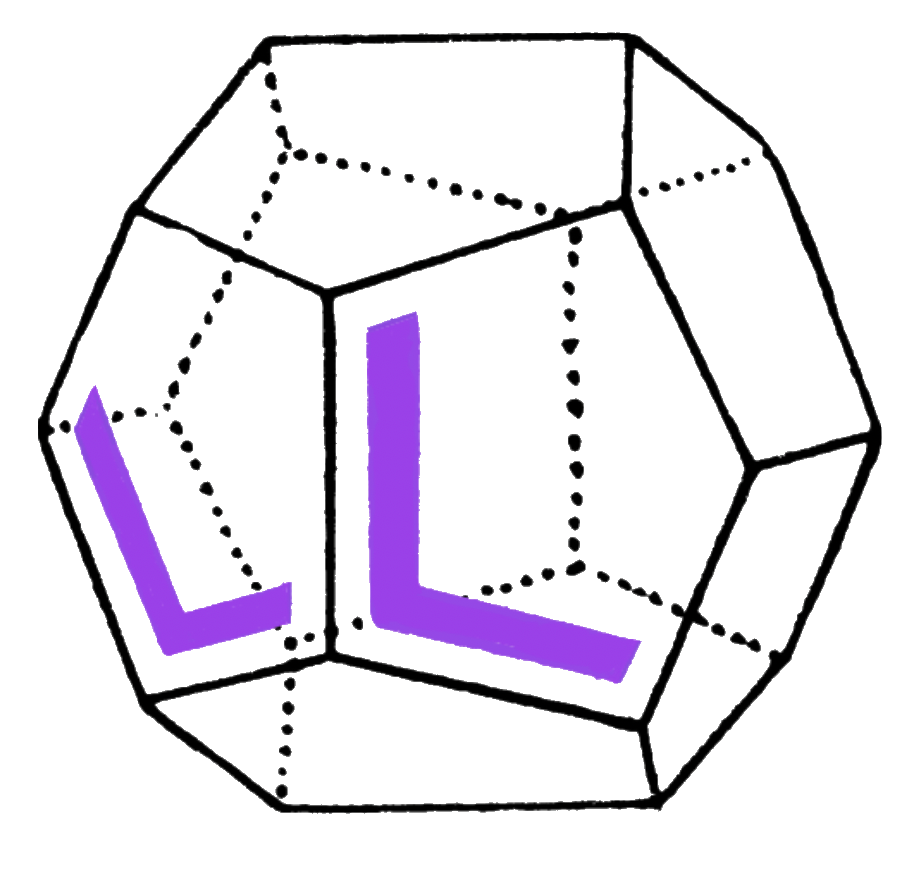
\includegraphics[width=2cm,height=2cm]{ll.png}}}}

\AddToShipoutPicture*
  {\put(465,767){\href{https://github.com/linlib/TheWhiteheadTheorem/blob/main/TheWhiteheadTheorem.py}{\raisebox{-0.198 em}{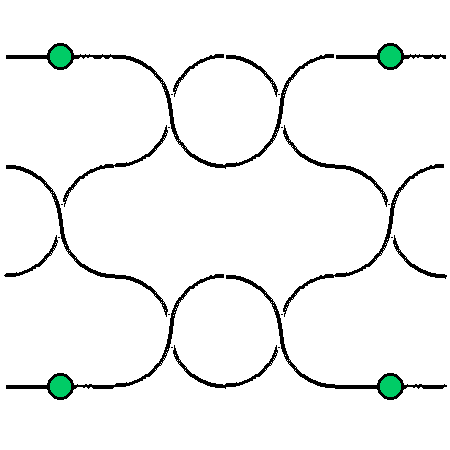
\includegraphics[width=0.35cm,height=0.35cm]{stringdiagrampicture.png}}\texttt{ Braid group}}
  }}

\AddToShipoutPicture*
  {\put(465,752){\href{https://ncatlab.org/nlab/show/HomePage}{\raisebox{-0.168 em}{
\includegraphics[width=0.33cm,height=0.33cm]{nlablogo.png}}\texttt{ nLab}}\\
  }}

\AddToShipoutPicture*
  {\put(465,737){\href{https://en.wikipedia.org/}{\texttt{\raisebox{-0.158 em}{
\includegraphics[width=0.38cm,height=0.30cm]{wikipedialogo.png}} Wikipedia}}\\
  }}

  \AddToShipoutPicture*
  {\put(465,722){\href{https://github.com/CQTS}{\texttt{\raisebox{-0.178 em}{
\includegraphics[width=0.32cm,height=0.32cm]{cqtslogo.png}} CQTS}}
  }}


\AddToShipoutPicture*
  {\put(375,767){\href{https://github.com/linlib/TheWhiteheadTheorem/blob/main/TheWhiteheadTheorem.lean}{\texttt{\raisebox{-0.1 em}{
\includegraphics[width=0.30cm,height=0.30cm]{leanlogo.png}} Lean file}}}}

\AddToShipoutPicture*
  {\put(375,752){\href{https://github.com/linlib/TheWhiteheadTheorem/blob/main/TheWhiteheadTheorem.agda}{\texttt{\raisebox{-0.09 em}{
\includegraphics[width=0.33cm,height=0.31cm]{agdalogo.png}} Agda file}}}}

\AddToShipoutPicture*
  {\put(375,737){\href{https://github.com/linlib/TheWhiteheadTheorem/blob/main/TheWhiteheadTheorem.v}{\texttt{\raisebox{-0.17 em}{
\includegraphics[width=0.31cm,height=0.34cm]{coqlogo.png}} Coq file}}}}

  \AddToShipoutPicture*
  {\put(375,722){\href{https://github.com/linlib/TheWhiteheadTheorem/blob/main/TheWhiteheadTheorem.thy}{\texttt{\raisebox{-0.2 em}{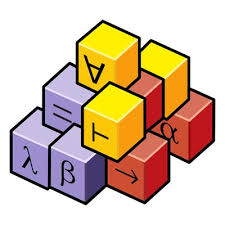
\includegraphics[width=0.34cm,height=0.35cm]{isabellelogo.png}} Isabelle file}}}}


\AddToShipoutPicture*
  {\put(281,767){\href{https://leanprover.zulipchat.com/}{\texttt{\raisebox{-0.1 em}{
\includegraphics[width=0.30cm,height=0.30cm]{leanlogo.png}} Lean Zulip}}}}

\AddToShipoutPicture*
  {\put(281,752){\href{https://agda.zulipchat.com}{\texttt{\raisebox{-0.09 em}{
\includegraphics[width=0.33cm,height=0.31cm]{agdalogo.png}} Agda Zulip}}\\
  }}

\AddToShipoutPicture*
  {\put(281,737){\href{https://coq.zulipchat.com}{\texttt{\raisebox{-0.17 em}{
\includegraphics[width=0.31cm,height=0.34cm]{coqlogo.png}} Coq Zulip}}\\
  }}

  \AddToShipoutPicture*
  {\put(281,722){\href{https://isabelle.zulipchat.com}{\texttt{\raisebox{-0.2 em}{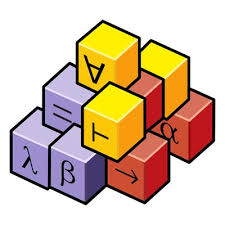
\includegraphics[width=0.34cm,height=0.35cm]{isabellelogo.png}} Isabelle Zulip}}
  }}


\AddToShipoutPicture*
  {\put(185,767){\href{https://linearlibrary.net}{\texttt{linearlibrary.net}}}}

\AddToShipoutPicture*
  {\put(185,752){\href{https://live.lean-lang.org}{\texttt{Leanprover}}}}

\AddToShipoutPicture*
  {\put(185,737){\href{https://github.com/linlib/TheWhiteheadTheorem/blob/main/TheWhiteheadTheorem.tex}{\texttt{Latex file}}
  }}

  \AddToShipoutPicture*
  {\put(185,722){\href{https://github.com/linlib/TheWhiteheadTheorem/blob/main/TheWhiteheadTheorem.pdf}{\texttt{PDF file}}
  }}

\ \\

\ \\
%LEAN: 
\begin{center}
\begin{tcolorbox}[width=5.8in,colback={white},coltitle=white]
\begin{center}
\ \\
\scalebox{3}{\texttt{The Whitehead Theorem}}\\
\end{center}
\end{tcolorbox}
\end{center}
\ \\


\ \\
%LEAN: 
\begin{center}
\begin{tcolorbox}[width=6in,colback={white}]
\begin{center}
\scalebox{0.85}{∀(C:D(∞-Cat)),∀(D:D(∞-Cat)),∀(F:D(∞-Cat).Hom C D),∀(G:D(∞-Cat).Hom C D),(∀(n:Nat),(Π⃗ₙ F = Π⃗ₙ G)) → F = G}\\
\ \\
\scalebox{0.85}{∀(X:D(∞-Grpd)),∀(Y:D(∞-Grpd)),∀(f:D(∞-Grpd).Hom X Y),∀(g:D(∞-Grpd).Hom X Y),(∀(n:Nat),(Πₙ f = Πₙ g)) → f = g}\\
\ \\
\scalebox{0.85}{∀(C:D(∞-Cat₋₁)),∀(D:D(∞-Cat₋₁)),∀(F:D(∞-Cat₋₁).Hom C D),∀(G:D(∞-Cat₋₁).Hom C D),(∀(n:Nat),(π⃗ₙ F = π⃗ₙ G)) → F = G}\\
\ \\
\scalebox{0.85}{∀(X:D(∞-Grpd₋₁)),∀(Y:D(∞-Grpd₋₁)),∀(f:D(∞-Grpd₋₁).Hom X Y),∀(g:D(∞-Grpd₋₁).Hom X Y),(∀(n:Nat),(πₙ f = πₙ g)) → f = g}\\
\end{center}
\end{tcolorbox}
\end{center}

\ \\
\begin{center}
\texttt{Plans to prove the Whitehead theorem}\\
\texttt{in Lean 4, with extensive use of Mathlib 4}
\end{center}
\ \\
\ \\


\thispagestyle{empty}

\iffalse
\newpage
\fi

\ \\
\ \\

\begin{center}

\pagecolor{white}
\color{black}

\end{center}

\thispagestyle{empty}

\newpage
\pagecolor{white}
\color{black}
\ \\
\ \\
\thispagestyle{empty}
\large %%%%%%%% HERE IS THE large LARGE size textsize set text size
\newpage 
\ \\
\ \\
\ \\
\ \\
\ \\
\ \\
\ \\
\ \\
\ \\
\ \\
\ \\
\thispagestyle{empty}
 
\newpage



\newpage

\ \\
\ \\
\ \\
\ \\
\ \\
\ \\
\ \\
\ \\
\ \\
\ \\
\ \\

We wish to acknowledge the collaborative efforts of Jiazhen Xia and E. Dean Young. Together the authors are pursuing these plans as a long term project.\\



\newpage
\section{Unicode}

Here is a list of the unicode characters we will use:

{\footnotesize
\begin{center}
\begin{tabular}{|| l || l || l || l ||} 
\hline
$\texttt{Symbol}$ & $\texttt{Unicode}$ & \texttt{VSCode shortcut} & $\texttt{Use}$\\
\hline
\hline
\multicolumn{4}{||c||}{\texttt{Lean's Kernel}} \\
\hline
\hline
× & 2A2F & \backslash\texttt{times} & Product of types\\
\hline
→ & 2192 & \backslash\texttt{rightarrow}  & Hom of types\\
\hline
⟨,⟩ & 27E8,27E9 & \backslash\texttt{langle},\backslash\texttt{rangle}  & Product term \\
\hline
↦ & 21A6 &\backslash\texttt{mapsto}  & Hom term \\
\hline
∧ & 2227 &\backslash\texttt{wedge}  & Conjunction \\
\hline
∨ & 2228 &\backslash\texttt{vee}  & Disjunction \\
\hline
∀ & 2200 &\backslash\texttt{forall}  & Universal quantification \\
\hline
∃ & 2203 &\backslash\texttt{exists}  & Existential quantification\\
\hline
¬ & 00AC &\backslash\texttt{neg}  & Negation\\
\hline
\hline
\multicolumn{4}{||c||}{\texttt{Variables and Constants}} \\
\hline
\hline
ᵃ,ᵇ,ᶜ,...,ᶻ & 1D52,1D56 & & Variables and constants \\
\hline
⁰,¹,²,³,⁴,⁵,⁶,⁷,⁸,⁹ & 1D52,1D56 &  & Variables and constants \\
\hline
⁻ & 207B &  & Variables and constants \\
\hline
₀,₁,₂,₃,₄,₅,₆,₇,₈,₉ & 2080 - 2089 & \backslash\texttt{0}-\backslash\texttt{9} & Variables and constants\\
\hline
𝔸,...,ℤ & 1D538 &  &  \\
\hline
𝕒,...,𝕫 & 1D552 &  &  \\
\hline
𝐀,...,𝐙 & 1D41A &  &  \\
\hline
𝐚,...,𝐳 & 1D41A &  &  \\
\hline
\texttt{α}-\texttt{ω},\texttt{A}-\texttt{Ω} & 03B1-03C9 & & Variables and constants\\
\hline
\hline
\multicolumn{4}{||c||}{\texttt{Categories}} \\
\hline
\hline
 𝟙 & 1D7D9 & \backslash\texttt{b1}  & The identity morphism\\
\hline
 ∘ & 2218 & \backslash\texttt{circ}  & Composition\\
 \hline
 \hline
 \multicolumn{4}{||c||}{\texttt{Bicategories}} \\
 \hline 
 \hline
 • & 2022  & \backslash\texttt{smul}  & Horizontal composition of objects\\ 
  \hline
  \hline
 \multicolumn{4}{||c||}{\texttt{Adjunctions}} \\
\hline
\hline
⇄ & 21C4 & \backslash\texttt{rightleftarrows}  & Adjunctions \\
\hline
⇆ & 21C6 & \backslash\texttt{leftrightarrows}  & Adjunctions \\
\hline
𛲔 & 1BC94 &  & Right adjoints\\
\hline
ॱ & 0971 &  & Left adjoints \\
\hline
⊣ & 22A3 & \backslash\texttt{dashv}  & The condition that two functors are adjoint \\
\hline
\hline
\multicolumn{4}{||c||}{\texttt{Monads and Comonads}} \\
\hline
\hline
?,¿ & 003F, 00BF & ?,\backslash\texttt{?}  & The corresponding (co)monad of an adjunction\\
\hline
!,¡ & 0021, 00A1 & !, \backslash\texttt{!}  & The (co)-Eilenberg-(co)-Moore adjunction \\
\hline
ꜝ,ꜞ & A71D, A71E &  & The (co)exponential maps\\
\hline
\hline
\multicolumn{4}{||c||}{\texttt{Miscellaneous}} \\
\hline
\hline
∼ & 223C & \backslash\texttt{sim} & Homotopies \\
\hline
≃ & 2243 & \backslash\texttt{equiv}  & Equivalences \\
\hline
≅ & 2245 & \backslash\texttt{cong}  & Isomorphisms \\
\hline
⊥ & 22A5 & \backslash\texttt{bot}  & The overobject classifier \\
\hline
∞ & 221E & \backslash\texttt{infty}  & Infinity categories and infinity groupoids\\ 
\hline
${}^{\leftrightarrow}$ & 20D7 &  & Homotopical operations on ∞-categories \\
\hline
${}^{\rightarrow}$ & 20E1 &  & Homotopical operations on ∞-groupoids \\
\hline
\end{tabular}
\end{center}}


\newpage
\section{Contents}



{
\footnotesize
\begin{longtable}{|| l || l ||} 
\hline
\multicolumn{1}{||c||}{$\texttt{Section}$} & \multicolumn{1}{|c||}{$\texttt{Description}$} \\
\hline
\hline
Unfinished & \\
\hline
Contents & \\
\hline
Unicode & \\
\hline
 & \\
\hline \hline
\multicolumn{2}{||c||}{\texttt{I: The Whitehead theorem for based CW-complexes}} \\
\hline \hline
\multicolumn{2}{||c||}{Based ∞-Groupoids} \\
\hline \hline
D(∞-Grpd₀) & The derived category of Based ∞-groupoids \\
\hline
D(∞-Grpd₀/X₀) & The derived category of Based ∞-groupoids over X₀. \\
\hline
Ω : ∞-Grpd₀ ⭢ ∞-Grpd & The loop space functor \\
\hline
Σ : ∞-Grpd₀ ⭢ ∞-Grpd₀ & The Based suspension functor \\
\hline 
ω f : ∞-Grpd/D₀ ⭢ ∞-Grpd/C₀ & The homotopy fiber\\
\hline 
σ f : ∞-Grpd₀/C₀ ⭢ ∞-Grpd₀/D₀ & Based homotopy pushout \\
 \hline 
πₙ : ∞-Grpd₀ ⭢ Set & The connected components functors\\
 \hline \hline
  \multicolumn{2}{||c||}{\texttt{The homotopy extension propertyThe Whitehead Theorem for Based ∞-Groupoids} \\
\hline \hline
Globular Sets & Defining globular sets\\
\hline
HEP for Based ∞-groupoids & The homotopy extension property for ∞$\texttt{-Grpd}$₀\\
 \hline 
REP for Based ∞-groupoids & The replacement functor on ∞$\texttt{-Grpd}$₀ \\
\hline
Whitehead theorem (c) & A map $\texttt{F : D(}$∞$\texttt{-Grpd₀).Hom E₀ B₀}$ is determined by $\texttt{λ(n:Nat),πₙ F}$. \\
\hline \hline
  \multicolumn{2}{||c||}{\texttt{Chapter 3: }The Category of Maps} \\
\hline \hline
HEP for Maps of Based ∞-groupoids & The homotopy extension property for ∞$\texttt{-Grpd}$₀\\
 \hline 
REP for Maps of Based ∞-groupoids & The replacement functor on ∞$\texttt{-Grpd}$₀ \\
\hline
The Whitehead theorem for Maps & ... \\
\hline \hline
\multicolumn{2}{||c||}{\texttt{II: } ∞-Groupoids} \\
\hline \hline 
\multicolumn{2}{||c||}{\texttt{Chapter 4: }∞\texttt{-Grpd}}\\
\hline \hline
D(∞-Grpd) & The derived category of ∞-groupoids \\
\hline
D(∞-Grpd/X) & The derived category of ∞-groupoids over X \\
\hline
Ω⃡ : ∞-Grpd ⭢ ∞-Grpd & The directed path space functor \\
 \hline 
Σ⃡ : ∞-Grpd ⭢ ∞-Grpd & The unBased suspension functor \\
 \hline 
ω⃡ f : ∞-Grpd⁄D ⭢ ∞-Grpd/C & The directed homotopy pullback functor\\
\hline 
σ⃡ f : ∞-Grpd/C ⭢ ∞-Grpd/D & Homotopy pushout with a point \\
 \hline 
Πₙ : ∞-Grpd ⭢ Set & The connected components functors\\
 \hline \hline
 \multicolumn{2}{||c||}{\texttt{Chapter 5: }The Whitehead Theorem for ∞-Groupoids} \\
\hline \hline
Cubical Complexes & ...\\
\hline
REP for ∞-groupoids & The cofibrant replacement functor for ∞-groupoids\\
\hline
HEP for ∞-groupoids & The homotopy extension property\\
\hline
Whitehead theorem (b) & A map $\texttt{F : D(}$∞$\texttt{-Grpd).Hom E B}$ is determined by $\texttt{λ(n:Nat),}$Πₙ
$\texttt{F}$. \\
\hline \hline
\multicolumn{2}{||c||}{\texttt{Chapter 6: }The Category of Maps of ∞-Groupoids} \\
\hline \hline
... & ...\\
\hline
REP for Maps of ∞-groupoids & The replacement functor on ∞$\texttt{-Grpd}$ \\
\hline
HEP for Maps of ∞-groupoids & The homotopy extension property for ∞$\texttt{-Grpd}$\\
 \hline 
The Whitehead theorem for Maps of ∞-groupoids & ... \\
\hline \hline
\multicolumn{2}{||c||}{\texttt{II: } Based ∞-CATEGORIES} \\
\hline \hline 
\multicolumn{2}{||c||}{\texttt{Chapter 4: }∞\texttt{-...}}\\
\hline \hline
D(∞-Grpd) & The derived category of ∞-groupoids \\
\hline
D(∞-Grpd/X) & The derived category of ∞-groupoids over X \\
\hline
Ω⃡ : ∞-Grpd ⭢ ∞-Grpd & The directed path space functor \\
 \hline 
Σ⃡ : ∞-Grpd ⭢ ∞-Grpd & The unBased suspension functor \\
 \hline 
ω⃡ f : ∞-Grpd⁄D ⭢ ∞-Grpd/C & The directed homotopy pullback functor\\
\hline 
σ⃡ f : ∞-Grpd/C ⭢ ∞-Grpd/D & Homotopy pushout with a point \\
 \hline 
Πₙ : ∞-Grpd ⭢ Set & The connected components functors\\
 \hline \hline
 \multicolumn{2}{||c||}{\texttt{Chapter 5: }The Whitehead Theorem for ∞-Groupoids} \\
\hline \hline
Cubical Complexes & ...\\
\hline
REP for ∞-groupoids & The cofibrant replacement functor for ∞-groupoids\\
\hline
HEP for ∞-groupoids & The homotopy extension property\\
\hline
Whitehead theorem (b) & A map $\texttt{F : D(}$∞$\texttt{-Grpd).Hom E B}$ is determined by $\texttt{λ(n:Nat),}$Πₙ
$\texttt{F}$. \\
\hline \hline
\multicolumn{2}{||c||}{\texttt{Chapter 6: }The Category of Maps of ∞-Groupoids} \\
\hline \hline
... & ...\\
\hline
REP for Maps of ∞-groupoids & The replacement functor on ∞$\texttt{-Grpd}$ \\
\hline
HEP for Maps of ∞-groupoids & The homotopy extension property for ∞$\texttt{-Grpd}$\\
 \hline 
The Whitehead theorem for Maps of ∞-groupoids & ... \\
\hline \hline
 \multicolumn{2}{||c||}{\texttt{III: } ∞-Categories} \\
\hline \hline
\multicolumn{2}{||c||}{\texttt{Chapter 7: }∞\texttt{-Cat}} \\
\hline \hline
D(∞-Cat) & The derived category of ∞-categories \\
\hline
D(∞-Cat⁄C) & The derived category of ∞-categories over C \\
\hline
Ω⃗ : ∞-Cat ⭢ ∞-Cat & The directed path space functor \\
 \hline 
 Σ⃗ : ∞-Cat ⭢ ∞-Cat & The directed unBased suspension \\
\hline 
ω⃗ f : ∞-Cat⁄D ⭢ ∞-Cat/C & The directed homotopy pullback functor\\
 \hline 
 σ⃗ f : ∞-Cat/C ⭢ ∞-Cat/D & The directed homotopy pushout \\
 \hline 
Π⃗ₙ : ∞-Cat ⭢ Set & The connected components functors\\
 \hline \hline
 \multicolumn{2}{||c||}{\texttt{Chapter 8: }The Whitehead Theorem for ∞-Categories} \\
\hline \hline
Directed Cubical Complexes & ...\\
\hline
REP for ∞-categories & The cofibrant replacement functor for ∞-categories\\
\hline
HEP for ∞-categories & The directed homotopy extension property\\
\hline 
Whitehead theorem (a) & A map $\texttt{F : D(}$∞$\texttt{-Cat).Hom E B)}$ is determined by $\texttt{λ(n:Nat),}$Π⃗ₙ$\texttt{F}$.\\
\hline \hline
\multicolumn{2}{||c||}{\texttt{Chapter 9: }The Category of Maps of ∞-Categories} \\
\hline \hline
REP for Maps of ∞-groupoids & The replacement functor on ∞$\texttt{-Grpd}$ \\
\hline
HEP for Maps of ∞-groupoids & The homotopy extension property for ∞$\texttt{-Grpd}$\\
 \hline 
The Whitehead theorem for Maps of ∞-groupoids & ... \\
\hline \hline
 \multicolumn{2}{||c||}{\texttt{IV: } A${}^{\infty}$ OPERADS AND OPEROIDS} \\
\hline \hline
 &  \\
\hline \hline
 \multicolumn{2}{||c||}{\texttt{V: } THE MODEL STRUCTURES ON □ ∞-Grpd and □ ∞-Cat} \\
\hline \hline
 & \\
\hline \hline
\multicolumn{2}{||c||}{\texttt{I: } ∞-SPACES} \\
\hline \hline
 \multicolumn{2}{||c||}{\texttt{Chapter 1: }Abelian Groups} \\
\hline \hline
abeliangroup & The type of abelian groups \\
\hline
Maps of abelian groups & Constructing homomorphisms of abelian groups \\
\hline
Negation & \\
\hline
The Eckman-Hilton Argument & \\
\hline
AbelianGroup ⭢ Group & The forgetful functor from abelian groups to groups \\
\hline
Eilenberg-Maclane Spaces & \\
\hline
Chain Complexes & \\
\hline
Realization of Chain Complexes & \\
\hline
Tensor Product of Chain Complexes & \\
\hline \hline
 \multicolumn{2}{||c||}{\texttt{Chapter 2: }∞-Spaces} \\
\hline \hline
∞-space & The type of ∞-spaces \\
\hline
Maps of ∞-spaces & Constructing maps of ∞-spaces \\
\hline
Negation & \\
\hline
The Eckman-Hilton Argument & \\
\hline
OperadicGroup OperadicGroup ∞-Grpd₋₁ ⭢ OperadicGroup ∞-Grpd₋₁ & \\
\hline
B¹ and Bⁿ & \\
\hline
[E⃗.obj ℕ, -] & Internal Complexes \\
\hline
Realization of Chain Complexes & \\
\hline
Tensor Product of Chain Complexes & \\
\hline \hline
\multicolumn{2}{||c||}{\texttt{Chapter 3: }Tensor Product of Abelian Groups} \\
\hline \hline
- ⊗\_(AbelianGroups) - & Mathlib's tensor product of abelian groups \\
\hline
[-,-]\_(AbelianGroups) & Mathlib's hom of abelian groups\\
\hline
AbelianGroup & The symmetric monoidal category of abelian groups\\
\hline \hline
\multicolumn{2}{||c||}{\texttt{Chapter 4: }Tensor Product of ∞-Spaces} \\
\hline \hline
- ⊗\_(∞-Space) - &  \\
\hline
[-,-]\_(∞-Space) &  \\
\hline
∞-Space & The symmetric monoidal category of ∞-spaces \\
\hline \hline
 \multicolumn{2}{||c||}{\texttt{Chapter 5: }Set₋₁ ⇄ AbelianGroups} \\
\hline \hline
??? & The free abelian group functor \\
 \hline
??? & The forgetful functor from abelian groups to pointed sets \\
 \hline
??? : Set₋₁ ⇄ AbelianGroup : ??? & The adjunction between pointed sets and abelian groups \\
\hline \hline
 \multicolumn{2}{||c||}{\texttt{Chapter 6: }∞-Grpd₋₁ ⇄ ∞-Space} \\
\hline \hline
??? & The free ∞-space given a Based ∞-groupoid \\
\hline
??? & The forgetul functor from ∞-spaces to ∞-groupoids \\
\hline
??? : ∞-Grpd₋₁ ⇄ ∞-Space : ??? & The ??? between ∞-Grpd₋₁ and ∞-Spaces \\
\hline \hline
\multicolumn{2}{||c||}{\texttt{II: } RINGS, COMMUTATIVE RINGS, A${}^{\infty}$-RINGS, AND E${}^{\infty}$-RINGS} \\
\hline \hline
\multicolumn{2}{||c||}{\texttt{Chapter 7: }Rings and Commutative Rings} \\
\hline \hline
ring & The type of rings \\
 \hline
Ring & The category of rings \\
\hline
commutative\_ring & The type of commutative rings  \\
\hline
CommutativeRing & The category of commutative rings \\
 \hline \hline
  \multicolumn{2}{||c||}{\texttt{Chapter 8: }A${}^{\infty}$-Rings and E${}^{\infty}$-Rings} \\
\hline \hline
A${}^{\infty}$-ring & The type of A${}^{\infty}$-rings \\
\hline
A${}^{\infty}$-Ring & The category of A${}^{\infty}$-Rings \\
 \hline
E${}^{\infty}$-ring  & The type of E${}^{\infty}$-rings \\
 \hline
E${}^{\infty}$-Ring  & The category of E${}^{\infty}$-Rings \\
 \hline \hline
\multicolumn{2}{||c||}{\texttt{Chapter 9: }Modules and Modules over Commutative Rings} \\
\hline \hline
 &  \\
 \hline
 &  \\
 \hline
InternalMonoidAction (InternalMonoid C) ≅ InternalMonoid (InteralMonoidAction C) & The ??? theorem \\ 
\hline
CommutativeAlgebra : CommutativeRing → Cat & The category of commutative algebras \\
\hline
Maps (Algebra A) : Cat & The category of maps of commutative A-algebras \\
\hline \hline
\multicolumn{2}{||c||}{\texttt{Chapter 10: }A${}^{\infty}$-Modules and E${}^{\infty}$-Modules} \\
\hline \hline
 &  \\
\hline
 &  \\
\hline
$A{}^{\infty}$-RingAction ($A{}^{\infty}$-Ring C) ≅ $A{}^{\infty}$-Ring ($A{}^{\infty}$-RingAction C) & The ??? theorem \\ 
\hline
Maps A${}^{\infty}$-Algebras & \\
 \hline \hline
\end{longtable}
}



\newpage
\section{Notes}

{\bf The main goal of this repository is to prove the Whitehead theorem in Lean 4 using Mathlib 4's homotopy groups}.\\

\iffalse
\item ℝ and ℚ, and also [0,∞], are supposed to be available as cohomology rings and or "a cohomology rig"
\item ℚ as colimitₙ ℤ[n!⁻¹] in internal abelian groups in Set
\item ℚ as colimitₙ ℤ[n!⁻¹] in internal abelian groups in locally compact locales (it's filtered!)
\item NNQ as colimitₙ ℕ[n!⁻¹] in internal commutative monoids in Set
\item NNQ as colimitₙ ℕ[n!⁻¹] in internal commutative monoids in locally compact locales (it's filtered!)
\item a * n!⁻ʲ = b * n!⁻ᵏ when a * n!ᵏ - b * n!ʲ = 0.
\item [0,∞) as the image of ⟨-,-⟩ ∘ Δ for any n
\item ℝⁿ as a locale using n!⁻¹
\item and 2-norm completion
\fi


Three other subsequent goals are to state and prove three variations of the Whitehead theorem, making four Whitehead theorems:\\

\begin{enumerate}[(a)]
\item (The Whitehead theorem for Based ∞-groupoids) ∀(E:D(∞-Grpd₋₁)),∀(B:D(∞-Grpd₋₁)),∀(F:D(∞-Grpd₋₁).Hom E B),∀(G:D(∞-Grpd₋₁).Hom E B),(∀(n:Nat),(πₙ F = πₙ G)) → F = G, where πₙ is notation for π n, where π n : Functor D(∞-Grpd₋₁) Set.
\item (The Whitehead theorem for ∞-groupoids) ∀(E:D(∞-Grpd)),∀(B:D(∞-Grpd)),∀(F:D(∞-Grpd).Hom E B),∀(G:D(∞-Grpd).Hom E B),(∀(n:Nat),(Ho ∘ [I,-]ⁿ F = Ho ∘ [I,-]ⁿ  G)) → F = G, where Πₙ is notation for Π n, where Π n : Functor D(∞-Grpd) Set.
\item (The Whitehead theorem for Based ) ∀(E:D(∞-Cat₋₁)),∀(B:D(∞-Cat₋₁)),∀(F:D(∞-Cat₋₁).Hom E B),∀(G:D(∞-Cat₋₁).Hom E B),(∀(n:Nat),(π⃗ₙ F = π⃗ₙ G)) → F = G, where π⃗ₙ is notation for π⃗ n, where π⃗ n : Functor D(∞-Cat₋₁) Set.
\item (The Whitehead theorem for ∞-categories) ∀(E:D(∞-Cat)),∀(B:D(∞-Cat)),∀(F:D(∞-Cat).Hom E B),∀(G:D(∞-Cat).Hom E B),(∀(n:Nat),(Ho ∘ [I⃗,-]ⁿ F = Π⃗ₙ G)) → F = G, where Ho ∘ [I⃗,-]ⁿ : Functor D(∞-Cat₋₁) Set ... 
\end{enumerate}

(a) in the above reflects the known Whitehead theorem, which dates back to Whitehead's two papers titled `Combinatorial Homotopy I' and `Combinatorial Homotopy II'. We will use two models of each of the following categories in the theorems above:

\begin{enumerate}[(i)]
\item We model ∞-Grpd₋₁ : Cat using based CW-complexes.
\item We model ∞-Grpd : Cat using CW-complexes.
\item We model ∞-Cat₋₁ : Cat using based directed CW-complexes.
\item We model ∞-Cat : Cat using directed CW-complexes.
\end{enumerate}

This choice accords with the standard approach to the third theorem, in which one typically chooses both a combinatorial and point-set model, with the former featuring a \href{https://github.com/leanprover-community/mathlib4/blob/8666bd82efec40b8b3a5abca02dc9b24bbdf2652/Mathlib/AlgebraicTopology/SimplicialSet.lean#L235-L236}{geometric realization functor} into the latter.\\

The theorems in the above involve the four pi-functors:

\begin{enumerate}[(i)]
\item πₙ : Functor D(∞-Grpd₋₁) Set
\item π⃗ₙ : Functor D(∞-Cat₋₁) Set
\item Ho ∘ [I,-]ⁿ : Functor D(∞-Grpd) Set
\item Ho ∘ [I⃗,-]ⁿ : Functor D(∞-Cat) Set
\end{enumerate}

While the functors πₙ occuring in the main theorems above are already defined in $\texttt{Mathlib 4}$ for topological spaces, the functors π⃗ₙ, Πₙ, and Π⃗ₙ are not. We will also form their derived functors:

\begin{enumerate}[(i)]
\item D(πₙ) : Functor D(∞-Grpd₋₁) Set
\item D(π⃗ₙ) : Functor D(∞-Cat₋₁) Set
\item Ho ∘ [I⃗,-]ⁿ : Functor D(∞-Grpd) (Map Set)
\item Ho ∘ [I⃗,-]ⁿ : Functor D(∞-Cat) (Map Set)
\end{enumerate}

In the course of the repository we will need the directed path space, path space, and loop space functors as well, which fit with the analogy formed by the Whitehead theorem and its two variations:

\begin{enumerate}
\item Ω : Functor ∞-Grpd₋₁ ∞-Grpd₋₁
\item Ω⃗ : Functor ∞-Cat₋₁ ∞-Cat₋₁
\item Ho ∘ [I⃗,-]ⁿ : Functor ∞-Grpd ∞-Grpd
\item Ho ∘ [I⃗,-]ⁿ : Functor ∞-Grpd ∞-Grpd
\end{enumerate}

Where γ is the unit interval and γ⃗ is the directed unit interval.\\

\iffalse
The latter, developed first, features a deformation retraction γ⃗ $\leftrightarrow$ γ⃗² between the directed unit interval and its cartesian product with itself.\\
\fi

\iffalse
In the directed context, a homotopy between two maps in ∞-Cat⁄C consists of a sequence of compatible directed homotopies with the odd morphisms in the sequence formed from reversed copies of Δ¹. Really we have two such categories, one of which consists of formal words, and another which involves ∞-categories and ∞-functors in the image of $\texttt{repl}$).\\

The main technical feature in the proofs of these theorems concerns a lifting property which successively lifts a homotopy along a single attachment of Δⁿ along its boundary ∂Δⁿ. A homotopy h : ∂Δⁿ × Δ¹ ⭢ Y between f, g : ∂Δⁿ ⭢ Y extends to a map H : Δⁿ × Δ¹ ⭢ Y. The directed case requires an extra technical feature. H(-,1) and g match on ∂Δⁿ, producing a map f : X ⭢ Y, where X consists of two copies of Δⁿ glued together at the boundary.\\

Consider a space X' formed as a quotient of Δⁿ × Δ¹ by ∂Δⁿ × Δ¹. There is a map φ : X ⭢ X'. An induction hypothesis on f and g involving πₙ ensures that the aparent map X ⭢ Y lifts along φ, producing a map from Δⁿ × Δ¹ which is constant on ∂Δⁿ × Δ¹. Stacking this on top of H can be done using an isomorphism between Δ¹ and Δ¹ glued with itself along different endpoints. Altogether this produces a homotopy between f and g.\\

We will define three different kinds of derived category:\\

\begin{enumerate}
\item D(∞-Cat) : Cat (the directed derived category of ∞-categories)
\item D(∞-Grpd) : Cat (the derived category of ∞-groupoids)
\item D(∞-Grpd₀) : Cat (the derived category of Based ∞-groupoids)
\end{enumerate}

We then create the second kind of derived category, one for each of the objects in the respective categories above:

\begin{enumerate}
\item For C : D(∞-Cat), a category D(∞-Cat/C) : Cat
\item For G : D(∞-Grpd), a category D(∞-Grpd/G) : Cat
\item For G₀ : D(∞-Grpd₀), a category D(∞-Grpd₀/G₀) : Cat
\end{enumerate}

For the model built on simplicial sets, Ω⃗ will be representable by Δ¹ with respect to an internal hom, and Ω⃡ will be representable by a model of the unit interval I := [0,1].\\

We will use six (strict) ``internal'' structures in addition to the standard structures in category theory:

\begin{enumerate}[(i)]
\item InternalCategory : Cat → Cat 
\item InternalPresheaf : (X : Cat) → (C : (InternalCategory X)) → Cat
\item InternalGroupoid : Cat → Cat
\item InternalGroupoidAction : (X : Cat) → (G : (InternalGroupoid X)) → Cat
\item InternalGroup : Cat → Cat
\item InternalGroupAction : (X : Cat) → (G₀ : (InternalGroup X)) → Cat   
\end{enumerate}

The book ``Galois theories" by Borceux and Janelidze contains the internal structures (iii), (iv), (v), and (vi), and the first two internal structures have fewer entries. That book details how to think about Galois theory using internal groupoids, internal G-presheaves, monadicity, comonadicity, and the constructions involved in Eilenberg-Moore theory.\\

Some previous work done on these structures can be found at the thread \href{https://leanprover.zulipchat.com/#narrow/stream/116395-maths/topic/Internal.20categories}{here}.\\

The six internal structures above arise here in relation to six functors:

\begin{enumerate}[(I)]
\item Ω⃗ : ∞-Cat ⭢ ∞-Cat (notation for the directed path space functor, related to [Δ¹,-]). D(Ω⃗) factors through internal categories in D(∞-Cat) by a categorical equivalence D(∞-Cat) ≅ InternalCategory D(∞-Cat) (internal categories in D(∞-Cat))
\item ω⃗ (𝟙 C) : ∞-Cat/C ⭢ ∞-Cat/C, the derived directed homotopy pullback with 𝟙 C. D(ω⃗ (𝟙 C)) factors through a categorical equivalence between D(∞-Cat/C) and internal P⃗C-presheaves in D(∞-Cat/C).
\item Ω⃡ : ∞-Grpd ⭢ ∞-Grpd (notation for the path space functor [I,-]), the derived homotopy pullback of an ∞-groupoid with itself. D(Ω⃡) factors through a categorical equivalence between D(∞-Grpd) and internal groupoids in D(∞-Grpd)
\item ω⃡ (𝟙 X) : ∞-Grpd/X ⭢ ∞-Grpd/X, the derived homotopy pullback with 𝟙 X. D(ω⃡ (𝟙 X)) factors through internal P⃡X
\item Ω : ∞-Grpd₀ ⭢ ∞-Grpd₀, the loop space functor. D(Ω) factors through a categorical equivalence between D(∞-Grpd₀) and internal groups in D(∞-Grpd₀) (the loop space functor on connected Based ∞-groupoids)
\item ω (𝟙 X) : ∞-Grpd₀/X₀ ⭢ ∞-Grpd₀/X₀, the homotopy pullback with the base of X₀. D(ω (𝟙 X)) factors through internal PX₀-actions in Based spaces over X₀.
\end{enumerate}

(v) in the above is shown \href{https://mathoverflow.net/questions/128883/why-omega-x-and-bg-are-adjoint-functors}{here} and (vi) in the above is shown in a typical exposition of $G$-principal bundles.\\

The functors ω⃗ (𝟙 C), ω⃡ (𝟙 X), and ω (𝟙 C) in the above ensue from a more general construction:\\

\begin{enumerate}
\item For C, D : D(∞-Cat), and f : C ⭢ D, ω⃗ f : D(∞-Cat/D) ⭢ D(∞-Cat/C)   (derived directed homotopy pullback)
\item For B, E : D(∞-Grpd), and f : E ⭢ B, ω⃡ f : D(∞-Grpd/B) ⭢ D(∞-Grpd/E) (derived homotopy pullback)
\item For B₀, E₀ : D(∞-Grpd₀), and f : E₀ ⭢ B₀, ω f : D(∞-Grpd₀/B₀) ⭢ D(∞-Grpd₀/E₀) (homotopy pullback with the base)
\end{enumerate}

These six factored functors P⃗ , P⃡ , P : D(∞-Grpd₀), p⃗ (𝟙 C), p⃡ (𝟙 X), p are each fully faithful and produce categorical equivalences; we later construct functors B⃗, B⃡, B, b⃗, b⃡, b defined on the essential image of these six, which are inverse to them up to natural isomorphism.\\

We obtain six categorical equivalences witnessed by these twelve functors (along with twelve natural isomorphisms). Here are the types of P⃗ , P⃡ , P : D(∞-Grpd₀), p⃗ (𝟙 C), p⃡ (𝟙 X), p:

\begin{enumerate}
\item The directed path space, the path space, and loop space form components of the functors P⃗, P⃡, and P, which are valued in internal categories, internal groupoids, and internal groups respectively.
\begin{enumerate}
\item P⃗ : D(∞-Cat) ⭢ Cat D(∞-Cat)
\item P⃡ : D(∞-Grpd) ⭢ Grpd D(∞-Grpd)
\item P : D(∞-Grpd₀) ⭢ Grp D(∞-Grpd) (see \href{https://mathoverflow.net/questions/128883/why-omega-x-and-bg-are-adjoint-functors}{here})
\end{enumerate}
\item The directed homotopy pullback, the homotopy pullback, and the homotopy pullback with the base form components of the functors Alg(Mon(ω⃗)), Alg(Mon(ω⃡)), and Alg(Mon(p)), respectively. 
\begin{enumerate}
\item p⃗ (𝟙 C) : D(∞-Cat⁄C) ⭢ InternalPresheaf D(∞-Cat⁄C) P⃗.obj C 
\item p⃡ (𝟙 X) : D(∞-Grpd⁄X) ⭢ InternalGroupoidAction D(∞-Grpd⁄X) P⃡.obj X
\item p (𝟙 X₀) : D(∞-Grpd₀⁄X₀) ⭢ InternalGroupAction D(∞-Grpd₀⁄X₀) P.obj X₀
\end{enumerate}
\end{enumerate}

Above, the functors P⃗, P⃡, P, p⃗, p⃡, and p feature Ω⃗, Ω⃡, Ω, ω⃗, ω⃡, and ω in their components, and can be related to them using constructions from Eilenberg-Moore theory.\\
\fi

\iffalse
Interspersing one of the 6 omegas's in each of six operadic structures, which have the same number of entries as the six internal structures respectively. In the thirteen entry operadic category, one of the entries is an ordinary object in the category, analogous to the first of the thirteen entries of the internal category. The second entry, instead of featuring the ordinal 2 (the morphism component, which is the second of two entries in the category in question), features a sequence of objects in the category. The identity morphism Idn : Obj ⭢ Mor of the internal category with 13 entries (as opposed to the slightly more complex structure in which separate clauses assume the existence of the relevant pullbacks so as to create an endofunction of Cat) is analogous to a function also from O₀ to O₁, and two further entires are essentially shared by both as well: Dom and Cod. One difference occurs in the component of an internal category for the properties that Idn has, which in the operadic case is 
\fi

\iffalse
J : Nat → ∞-Grpd
\fi

\iffalse
Ω⃗, Ω⃡, Ω⃗₀, Ω⃡₀ are the ones I construct and Ω Mathlib's.
\fi

\iffalse
Adding in the operadic structures.
\fi


\iffalse
https://leanprover.zulipchat.com/#narrow/stream/116395-maths/topic/Internal.20categories
\fi

\iffalse
{
\footnotesize
\begin{center}
\begin{tabular}{||l || l || l || l ||} 
 \hline
  \multicolumn{4}{||c||}{\texttt{Twelve Structures}} \\
 \hline
 \multicolumn{2}{||c||}{\texttt{Strict}}  &  \multicolumn{2}{||c||}{\texttt{Lax}} \\
 \hline
 \texttt{Unitial} &  \texttt{Actional}  &  \texttt{Unitial} &  \texttt{Actional}\\
 \hline \hline
 \texttt{InternalCategory}  & \texttt{InternalPresheaf} & \texttt{OperadicCategory} & \texttt{OperadicPresheaf} \\ 
 \hline
 \texttt{InternalGroupoid} & \texttt{InternalGroupoidAction} & \texttt{OperadicGroupoid} & \texttt{OperadicGroupoidAction} \\ 
 \hline
\texttt{InternalGroup} & \texttt{InternalGroupAction} & \texttt{OperadicGroup} & \texttt{OperadicGroupAction} \\ 
 \hline 
\end{tabular}
\end{center}
}
\fi

\iffalse
{\footnotesize
\begin{center}
\scalebox{1.1}{
\begin{tabular}{|| l | l || l | l || } 
\hline
\hline
\multicolumn{2}{||c||}{Internal} & \multicolumn{2}{||c||}{Operadic} \\
\hline
\multicolumn{2}{||c||}{Unitial} & \multicolumn{2}{||c||}{Actional} & \multicolumn{2}{||c||}{Unitial} & \multicolumn{2}{||c||}{Actional} \\
\hline
\hline
$\texttt{InternalCategory : Cat → Cat}$ & $\texttt{InternalPresheaf : (C : Cat) → (InternalCategory C) → Cat}$ & $\texttt{OperadicCategory\_(-) : ∞-Cat\_(-) → ∞-Cat\_(-)}$ & OperadicPresheaf\_(-) : (X : ∞-Cat\_(-)) → ∞-Cat\_{(-)} \\
\hline
$\texttt{InternalGroupoid\_(-) : Cat\_(-) → Cat\_(-)}$ & $\texttt{InternalGroupoidAction : (C : Cat) → (InternalGroupoid C) → Cat}$& $\texttt{OperadicGroupoid\_(-) : ∞-Cat\_(-) → ∞-Cat\_(-)}$ & OperadicGroupoidAction\_(-) : (OperadicGroupoid\_() C) → (InternalCategory C) → ∞-Cat\_(-) → ∞-Cat\_(-) \\
\hline
$\texttt{InternalMonoid\_(-) : Cat\_(-) → Cat\_(-)}$ & $\texttt{InternalMonoidAction : (C : Cat) → (InternalMonoid C) → Cat}$ & $\texttt{OperadicMonoid\_(-) : ∞-Cat\_(-) → ∞-Cat\_(-)}$ & $\texttt{OperadicMonoidAction}$\_$\texttt{(-) : ∞-Cat\_(-) → ∞-Cat\_(-)}$\\
\hline
$\texttt{InternalGroup\_(-) : Cat\_(-) → Cat\_(-)}$ & $\texttt{InternalGroupAction : (C : Cat) → (InternalGroup C) → Cat}$ & $\texttt{OperadicGroup\_(-) : ∞-Cat\_(-) → ∞-Cat\_(-)}$ & $\texttt{OperadicGroupAction}$\_$\texttt{(-) : ∞-Cat\_(-) → ∞-Cat\_(-)}$\\
 \hline
\end{tabular}}
\end{center}}
\fi

\iffalse
\ \\
{\footnotesize
\begin{center}
\scalebox{1.1}{
\begin{tabular}{|| l || l ||} 
\hline
\hline
Ω⃗ : ∞-Cat ⭢ ∞-Cat & ω⃗ : (C : ∞-Cat) → (D : ∞-Cat) → (F : ∞-Cat.hom C D) → (∞-Cat⁄D) ⭢ ∞-Cat \\
\hline
O⃗ : ∞-Cat ⭢ OperadicCategory ∞-Cat & o⃗ : (C : ∞-Cat) → (D : ∞-Cat) → (F : ∞-Cat.hom C D) → (∞-Cat⁄D) ⭢ OperadicPresheaf (O⃗.obj D)\\
\hline
P⃗ : ∞-Cat ⭢ InternalCategory D(∞-Cat) & p⃗ : (C : ∞-Cat) → (D : ∞-Cat) → (F : ∞-Cat.hom C D) → (∞-Cat⁄D) ⭢ InternalPresheaf (P⃗.obj D) \\
\hline
\hline
Ω⃡ : ∞-Grpd ⭢ ∞-Grpd & ω⃡ : (X : ∞-Grpd) → (Y : ∞-Grpd) → (F : ∞-Cat.hom X Y) → (∞-Grpd⁄Y) ⭢ ∞-Grpd \\
\hline
O⃡ : ∞-Grpd ⭢ OperadicGroupoid ∞-Grpd & o⃡ : (X : ∞-Grpd) → (Y : ∞-Grpd) → (F : ∞-Cat.hom X Y) → (∞-Grpd⁄Y) ⭢ OperadicGroupoidAction (O⃡.obj Y) \\
\hline
P⃡ : ∞-Grpd ⭢ InternalGroupoid D(∞-Grpd) & p⃡ : (X : ∞-Grpd) → (Y : ∞-Grpd) → (F : ∞-Cat.hom C D) → (∞-Grpd⁄Y) ⭢ InternalGroupoidAction (P⃡.obj Y)  \\
\hline
\hline
Ω : ∞-Grpd₋₁ ⭢ ∞-Grpd₋₁  & ω : (X₋₁ : ∞-Grpd₋₁) → (Y₋₁ : ∞-Grpd₋₁) → (F : ∞-Grpd₋₁.hom X₋₁ Y₋₁) → (∞-Grpd₋₁⁄Y₋₁) ⭢ ∞-Grpd₋₁ \\
\hline
O : ∞-Grpd₋₁ ⭢ OperadicGroup ∞-Grpd₋₁ & o : (X₋₁ : ∞-Grpd₋₁) → (Y₋₁ : ∞-Grpd₋₁) → (F : ∞-Grpd₋₁.hom X₋₁ Y₋₁) → (∞-Grpd₋₁⁄Y₋₁) ⭢ OperadicGroupAction (O.obj X) \\
\hline
P : ∞-Grpd₋₁ ⭢ InternalGroup D(∞-Grpd₋₁) & p : (X₋₁ : ∞-Grpd₋₁) → (Y₋₁ : ∞-Grpd₋₁) → (F : ∞-Grpd₋₁.hom X₋₁ Y₋₁) → (∞-Grpd₋₁⁄Y₋₁) ⭢ InternalGroupAction (P.obj X₋₁) \\
\hline
 \hline
\end{tabular}}
\end{center}}

\fi


\begin{center}
\begin{tabular}{||c||c|c||c|c|}
\hline
\hline
  & \multicolumn{2}{||c||}{Enriched} & \multicolumn{2}{||c||}{Internal} \\
\hline
\hline
$\texttt{Strict Unitial}$  & enriched category & 7 entries & internal category & 13 entries \\ 
\hline
$\texttt{Strict Actional}$ & enriched presheaf & 3 entries & internal presheaf & 5 entries\\ 
\hline
\hline
$\texttt{A}^{\infty}$ $\texttt{Unitial}$  & enriched $A^{\infty}$-operoid & 7 entries & internal $A^{\infty}$-operoid action & 13 entries \\ 
\hline
$\texttt{A}^{\infty}$ $\texttt{Actional}$ & enriched $A^{\infty}$-operoid action & 3 entries & internal $A^{\infty}$-operad action & 5 entries \\ 
\hline
\hline
\end{tabular}
\end{center}



\newpage
\section{Unicode}

Here is a list of the unicode characters we will use:

{\footnotesize
\begin{center}
\begin{tabular}{|| l || l || l || l ||} 
\hline
$\texttt{Symbol}$ & $\texttt{Unicode}$ & \texttt{VSCode shortcut} & $\texttt{Use}$\\
\hline
\hline
\multicolumn{4}{||c||}{\texttt{Lean's Kernel}} \\
\hline
\hline
× & 2A2F & \backslash\texttt{times} & Product of types\\
\hline
→ & 2192 & \backslash\texttt{rightarrow}  & Hom of types\\
\hline
⟨,⟩ & 27E8,27E9 & \backslash\texttt{langle},\backslash\texttt{rangle}  & Product term \\
\hline
↦ & 21A6 &\backslash\texttt{mapsto}  & Hom term \\
\hline
∧ & 2227 &\backslash\texttt{wedge}  & Conjunction \\
\hline
∨ & 2228 &\backslash\texttt{vee}  & Disjunction \\
\hline
∀ & 2200 &\backslash\texttt{forall}  & Universal quantification \\
\hline
∃ & 2203 &\backslash\texttt{exists}  & Existential quantification\\
\hline
¬ & 00AC &\backslash\texttt{neg}  & Negation\\
\hline
\hline
\multicolumn{4}{||c||}{\texttt{Variables and Constants}} \\
\hline
\hline
ᵃ,ᵇ,ᶜ,...,ᶻ & 1D52,1D56 & & Variables and constants \\
\hline
⁰,¹,²,³,⁴,⁵,⁶,⁷,⁸,⁹ & 1D52,1D56 &  & Variables and constants \\
\hline
⁻ & 207B &  & Variables and constants \\
\hline
₀,₁,₂,₃,₄,₅,₆,₇,₈,₉ & 2080 - 2089 & \backslash\texttt{0}-\backslash\texttt{9} & Variables and constants\\
\hline
𝔸,...,ℤ & 1D538 &  &  \\
\hline
𝕒,...,𝕫 & 1D552 &  &  \\
\hline
𝐀,...,𝐙 & 1D41A &  &  \\
\hline
𝐚,...,𝐳 & 1D41A &  &  \\
\hline
\texttt{α}-\texttt{ω},\texttt{A}-\texttt{Ω} & 03B1-03C9 & & Variables and constants\\
\hline
\hline
\multicolumn{4}{||c||}{\texttt{Categories}} \\
\hline
\hline
 𝟙 & 1D7D9 & \backslash\texttt{b1}  & The identity morphism\\
\hline
 ∘ & 2218 & \backslash\texttt{circ}  & Composition\\
 \hline
 \hline
 \multicolumn{4}{||c||}{\texttt{Bicategories}} \\
 \hline 
 \hline
 • & 2022  & \backslash\texttt{smul}  & Horizontal composition of objects\\ 
  \hline
  \hline
 \multicolumn{4}{||c||}{\texttt{Adjunctions}} \\
\hline
\hline
⇄ & 21C4 & \backslash\texttt{rightleftarrows}  & Adjunctions \\
\hline
⇆ & 21C6 & \backslash\texttt{leftrightarrows}  & Adjunctions \\
\hline
𛲔 & 1BC94 &  & Right adjoints\\
\hline
ॱ & 0971 &  & Left adjoints \\
\hline
⊣ & 22A3 & \backslash\texttt{dashv}  & The condition that two functors are adjoint \\
\hline
\hline
\multicolumn{4}{||c||}{\texttt{Monads and Comonads}} \\
\hline
\hline
?,¿ & 003F, 00BF & ?,\backslash\texttt{?}  & The corresponding (co)monad of an adjunction\\
\hline
!,¡ & 0021, 00A1 & !, \backslash\texttt{!}  & The (co)-Eilenberg-(co)-Moore adjunction \\
\hline
ꜝ,ꜞ & A71D, A71E &  & The (co)exponential maps\\
\hline
\hline
\multicolumn{4}{||c||}{\texttt{Miscellaneous}} \\
\hline
\hline
∼ & 223C & \backslash\texttt{sim} & Homotopies \\
\hline
≃ & 2243 & \backslash\texttt{equiv}  & Equivalences \\
\hline
≅ & 2245 & \backslash\texttt{cong}  & Isomorphisms \\
\hline
⊥ & 22A5 & \backslash\texttt{bot}  & The overobject classifier \\
\hline
∞ & 221E & \backslash\texttt{infty}  & Infinity categories and infinity groupoids\\ 
\hline
${}^{\rightarrow}$ & 20E1 &  & Used for structures with r value of 1 \\
\hline
\hline
\end{tabular}
\end{center}}

Of these, the characters $\texttt{ꜝ,ꜞ,𛲔,ॱ}$,${}^{\rightarrow}$, and ${}^{\leftrightarrow}$ do not have VSCode shortcuts.\\

\ \\
\ \\
\ \\


\newpage
{
\Huge 
\begin{center}
\ \\
\ \\
\texttt{THE WHITEHEAD THEOREM}
\ \\
\ \\
\end{center}
\thispagestyle{empty}
}

\begin{center}
\texttt{∀(E:D(∞-Grpd₋₁)),∀(B:D(...)),∀(f:D(...).Hom E B),∀(G:D(∞-Grpd₋₁).Hom E B),(∀(n:Nat),(πₙ F = πₙ G)) → F = G}
\end{center}


\section{The homotopy extension property}

{\bf Definition:} (πₙ as a functor on spaces under 𝔻ⁿ).

\begin{enumerate}
\item Write $\partial_{\texttt{n}} : S^n \rightarrow D^n$ for the boundary of ...\\
\item Let $X$ be a CW-complex with $\text{Sk}_{n} X$ made from attaching maps $\phi_{n}
\item Let $\phi : D^n \rightarrow Y$, $\phi_n : D^n \rightarrow Y$ and $f_{n-1} : X \rightarrow \texttt{Y}$ be continuous maps such that $\pi_{\texttt{n}}(\phi^{\texttt{0}}_{\texttt{n}}) = \pi_{\texttt{n}}(\phi^{\texttt{1}}_{\texttt{n}})$.
\item Fix a continuous function $\psi : D^n \rightarrow X$ such that $\psi|_{S^{n}} = \phi_{\texttt{n}}^{\texttt{0}}|_{S^{n}} = \phi_{\texttt{n}}^{\texttt{0}}|_{S^{n}}$.
\item Define $f : S^n \rightarrow X$ via the UMP of pushout using the attaching map and $\psi$.
\item Where $\phi^{\texttt{0}}_{\texttt{n}} = \texttt{pushout} \partial_{\texttt{n}} \phi^{\texttt{0}} \rightarrow \texttt{Y}$ and $\phi^{\texttt{1}}_{\texttt{n}} = \texttt{pushout} \partial_{\texttt{n}} \texttt{f}_{\texttt{1}} \rightarrow \texttt{Y}$.
\item $\phi_n : D^n \rightarrow X$.
\item 
\end{enumerate}


 spaces under Sⁿ

Definition (spaces under Sⁿ): A space under Sⁿ is a pair (X, f) where X is a topological space and f : Dⁿ → X is a continuous function. A morphism of spaces under Sⁿ φ : (X,f) → (Y,g) is a continuous function h : X → Y such that g  ∘ ∂ₙ  = h ∘ f ∘ ∂ₙ.

Definition Write ∂ₙ for the continuous function from Sⁿ to Dⁿ sending a unit vector x with ||x||₂ = 1 to the (same) vector x, where we note that ||x||₂ = 1 implies ||x||₂ ≤ 1.

Definition (πₙ(-;-) as a functor on spaces under Sⁿ): Consider the category of Spc\Sⁿ of spaces under Sⁿ.

For an object (X,f) in Spc\Sⁿ, we can consider 

(1) the continuous function - ∘ ∂ₙ : [Dⁿ, X] → [Sⁿ, X] sending g to g ∘ ∂ₙ

(2) the continuous function c(f) : {*} → [Sⁿ,X] sending * to f

Define the pullback 

pullback (- ∘ ∂ₙ) c([Sⁿ,X], f)

As the topological space satisfying the UMP (universal mapping property) of pullback.

Keeping (X,f) in Spc\Sⁿ and writing Id for the identity function on the closed unit interval [0,1], we can consider

(1) the continuous function - ∘ (∂ₙ × Id) : [Dⁿ × [0,1], X] → [Sⁿ×  [0,1], X] sending g to g ∘ (∂ₙ × Id)

(2) the continuous function c = c([Sⁿ× Id, X] , f ∘ proj₀ ) : {*} → [Sⁿ× Id, X] sending * to the function f ∘ proj₀, where proj₀ : Sⁿ× Id → Sⁿ sends (x,t) to x.

Define the pullback 

pullback (- ∘ (∂ₙ × Id)) c

As the topological space satisfying the UMP (universal mapping property) of pullback.

For each t in the closed unit interval [0,1], there is a continuous function

evₜ : pullback (- ∘ (∂ₙ × Id)) c(f) → pullback (- ∘ (∂ₙ × Id)) 

We define πₙ(X;f) as the equilizer:

coeq ( ev₀, ev₁ )

Let X and Y be spaces and let φ : X  → Y be a continuous function... spaces X and Y under Sⁿ  πₙ(φ;f,g)


Definition (change of base for connected spaces under Dⁿ):  Let φ : X → Y be a continuous function between topological spaces X and Y, and let f₀, f₁ : Sⁿ → X and g₀, g₁ : Sⁿ → Y be continuous functions such that φ ∘ g₀ = f₀ and φ ∘ g₁ = f₁. Then πₙ(-;)  ...


Theorem (commutativity of base for connected spaces under Dⁿ): Let φ : X → Y be a continuous function between topological spaces X and Y, and let f : [0,1] × Sⁿ → X and g : [0,1] × Sⁿ → Y be continuous functions such that, setting Id : [0,1] → [0,1] as the (continuous) identity function, (Id × φ) ∘ f = g, defining the continuous functions fₜ : Sⁿ → X by fₜ(x) = f(t,x) and gₜ : Sⁿ → X by gₜ(x) = g(t,x), we have πₙ(φ;f₁,g₁)  ∘ trans(X,f) = trans(X,g) ∘ πₙ(φ;f₀,g₀) 

[Sⁿ,X] is the object component of a certain algebra for the 13-entry internal A-infinity operad of lines with Hom component [I × Sⁿ, X]. To transport a morphism of spaces under Sⁿ, we 


Theorem (The homotopy extension property for spaces under Dⁿ) Let (Skⁿ⁻¹ X, fₙ) be a space under Dⁿ, so that Skⁿ⁻¹ X is a topological space and fₙ : Dⁿ → Skⁿ⁻¹ X is a continuous function. Write Skⁿ X for the pushout 

pushout fₙ 

Let φ, ψ : Dⁿ → Y and φⁿ⁻¹, ψⁿ⁻¹ : Skⁿ⁻¹ X → Y be continuous functions with φⁿ⁻¹ = ψⁿ⁻¹ and define φⁿ, ψⁿ : Skⁿ X → Y as the pushouts

 φⁿ := pushout (φ ∘ ∂ₙ)  φⁿ⁻¹

ψⁿ := pushout (ψ ∘ ∂ₙ)  ψⁿ⁻¹

Suppose that πₙ(φⁿ) = πₙ(ψⁿ). Then φⁿ and ψⁿ are homotopic.

Proof: (Y, φⁿ ∘ fₙ) and (Y, ψⁿ ∘ fₙ)  are spaces under Dⁿ. and φⁿ and ψⁿ constitute maps of spaces under Dⁿ from (Skⁿ X,fₙ) to (Y, φⁿ ∘ fₙ) and from (Skⁿ X, fₙ) to (Y, ψⁿ ∘ fₙ) respectively. 


Theorem (Hatcher 0.16): 

 is the subspace of the compact open topology on the subset of the object component of [Dⁿ, X] consisting of f such that f ∘ ∂ₙ = φ ∘ ∂ₙ. Define [𝔻ⁿ



\section{The Whitehead theorem for based CW-complexes}


{\bf Theorem:} 



\section{The replacement functors Replₙ and the inclusion functors...}



\newpage
{
\Huge 
\begin{center}
\ \\
\ \\
\texttt{THE WHITEHEAD THEOREM FOR CW-COMPLEXES}
\ \\
\ \\
\end{center}
\thispagestyle{empty}
}

\iffalse

The Whitehead theorem is about the ways that spheres get trapped in spaces (higher homotopy groups), and the last section established how these higher homotopy groups relate to maps in the homotopy category of Based CW-complexes.\\

\section{Chapter 9: ∞\texttt{-Grpd}}


\subsection{- × I : ∞-Grpd ⇄ ∞-Grpd : [I,-]}

Our choice of symbols refects our choice of three variations of the Whitehead theorem and three Puppe sequences. Ω⃡, the analogue of loop space, is the internal hom functor [I,-] : ∞-Grpd ⭢ ∞-Grpd. This is not hard to construct, with the main lemma being that the path space of a quasicategory has the quasicategory lifting conditon.\\

We will be interested in one formal model of D(∞-Cat) which consists of formal compositions f₁ • g₁ • f₂ • g₂ • ⋯ • fₙ • gₙ, where gₙ $: Dom(f{}_{n+1}) $⭢ ??? is a weak equivalence, and something similar for D(∞-Cat). However, it is still vital to have the replacement functor $\texttt{repl}$, which ensures the Whitehead theorem for particular ∞-categories which are constructed out of attaching maps.\\


\subsection{??? : ⇄  : ???}

Ω⃗ is to internal categories as ω⃡ is to internal G-actions. It is also called directed homotopy pullback. These functors will later be used to produce functors P⃡ : D(∞-Grpd) ⭢ InternalCategory D(∞-Grpd) and p⃡ : D(∞-Grpd⁄C) ⭢ InternalPresheaf (P⃡ G) D(∞-Grpd⁄G).\\


\subsection{Πₙ : Functor ∞-Grpd Set}






\section{Chapter 10: The Whitehead Theorem for ∞-Groupoids}




\subsection{???}

...\\

\iffalse
In this chapter, we take on the objective of Whitehead theorem (a), out of which we will prove the other more concrete Whitehead theorems:\\

\begin{center} ∀(E:D(∞-Grpd)),∀(B:D(∞-Grpd)),∀(F:E ⭢ B),∀(G:E ⭢ B),(∀(n:Nat),(Πₙ F = Πₙ G)) ⭢ F = G
\end{center}

We can attempt to form a slightly different category, much like the above, called 𝓓(∞-Cat), at first, and in a formal way, so as to create a category whose object component 𝓓(∞-Cat).α matches the object component ∞-Cat.α while featuring the above theorem in a formal way. However, with this as our model of D(∞-Cat), we may then also be interested in the establishment of a model in which the Whitehead theorem is demonstrated, with the main idea being to prove two complementary concepts:

\begin{enumerate}
\item (REP) Establish ``weak equivalent fibrant replacement" R : ∞-Cat.α ⭢ ∞-Cat.α (.α gives the object component in Mathlib's category theory library), analogous to CW-complex replacement in Whitehead's original paper. It's especially nice if R forms the object component of a functor F : ∞-Cat ⭢ ∞-Cat. D(F) : D(∞-Cat) ⭢ D(∞-Cat) should be a categorical equivalence, and that is what we will do.
\item (HEP) For the object R X, demonstrate that any F,G : (R X) ⭢ Y such that ∀(n:Nat),(Π⃗ₙ F = Π⃗ₙ G), there is a directed homotopy equivalence between F and G. Note that ``directed homotopy equivalence" consists of a composible sequence of simple directed homotopies Hᵢ : Δ¹ × (R X) ⭢ Y, 1 ≤ i ≤ n, with even Hᵢ running reverse to the odd Hᵢ.
\end{enumerate} 

Both of these will use induction on Lean's $\texttt{Nat}$. The first of these could be called a REP (for REplacement Property, but this isn't usual terminology), and the second typically uses induction and a HEP (Homotopy Extension Property). Our REPa will consist of objects made out of particular kinds of pushouts called attaching maps, and can be made functorial. Proving the HEPa can be done by well-order induction on the attaching maps present in our choice of R, thereby reducing to the case of extending a homotopy along a single attachment.\\

Our HEPa (directed box filling) is similar to the HEP shown in Whitehead's original paper, and to the approach detailed in Hatcher's textbook, though no doubt modified to suit our two goals:

\begin{enumerate}[(I)]
\item The analogue of the Puppe sequence on the front cover needs to hold.
\item The first Whitehead theorem on the front cover needs to hold.
\end{enumerate}

These two considerations determine our choice of Π⃗ₙ, Ω⃗, and ω⃗. We take Ω⃗ to be (simply) the internal hom functor [Δ¹,-] (which requires showing that Ω⃗X has the inner-horn filling condition). ω⃗ is then defined as a certain pullback of Ω⃗, and Π⃗ₙ is designed to produce a Puppe sequence with a meaningful notion of exactness by which we can demonstrate the goal of recognition theorems (i) and (ii). Specifically, it makes sense to use cubes in our definition of Π⃗ₙ because of how they are representing objects of Ω⃗ⁿ. Meanwhile, it is also clear that the quotient producing Π⃗ₙ is subtle in exactly how it requires fixing the endpoints of a sequence of alternating directed homotopies. We will define Π⃗ₙ's by identifying those objects x, y: Ω⃗ⁿ X which are homotopic by a homotopy which restricts to a constant along the face maps fᵢ : Ω⃗${}^{n-1}$ X ⭢ Ω⃗${}^{n-1}$ X (which correspond to Maps (n,b), where b : Bool).\\

Imagine for a moment the picture of a square shaped cusion; we might make such a cusion by first soeing together 6 squares of cloth and filling it with material, then "soeing the walls down to a square". Here we go with this:

\begin{enumerate}
\item Define a n-cubical cusion using the boundary of an n-1 cube times Δ¹, i.e. the quotient of (Δ¹)${}^{n-1}$ × Δ¹ by an equivalence relation, but we have to start our model somewhere), or perhaps more easily the pushout of f : Δ¹ × (∂((Δ¹)ⁿ)) ⭢ (Δ¹)${}^{n+1}$ by the projection map Δ¹ × (∂((Δ¹)ⁿ)) ⭢ ∂((Δ¹)ⁿ)
\item Define a simplicial cusion using the boundary of an n-1 simplex times Δ¹, i.e. the quotient of (Δ¹) by an equivalence relation, or perhaps more easily the pushout of f : Δ¹ × (∂(Δⁿ)) ⭢ (Δ¹) × Δⁿ by the projection map Δ¹ × (∂((Δ¹)ⁿ)) ⭢ ∂(Δⁿ)
\end{enumerate}

The boundary of a cusion is a pouch, isomorphic to a pushout of two cubes glued together at their boundaries:

\begin{enumerate}
\item Define a n-cubical pouch as the pushout of two boundary maps ∂((Δ¹)ⁿ) ⭢ (Δ¹)ⁿ
\item Define a simplicial pouch as the pushout of two boundary maps ∂(Δⁿ) ⭢ Δⁿ
\end{enumerate}

Notice that paths in Ω⃗ⁿX produce paths in Ω⃗${}^{n-1}$X in as many ways as there are face maps (Δ¹)${}^{n-1}$ ⭢ Δ¹${}^{n}$, these could be called restrictions and are no doubt related to the pouches and cusions we just defined. The cartesian closed structure on simplicial sets with the lifting condition clarifies the relationship between the two available definitions of Π⃗ₙ:

\begin{enumerate}
\item Homotopies of maps from a cube which are constant on the boundary
\item Paths of maps in Ω⃗${}^{n-1}$X which produce constant maps under the mentioned restritions.
\item Maps from a pouch mod an equivalence relation (really we phrase this as a pushout!), namely the equivalence relation in which any two maps from a pouch that extend to maps from a cusion are identified.
\end{enumerate}

After we construct Π⃗ₙ in the first section, we will be in a place to demonstrate that the natural transformation $\texttt{weak\_equivalence : repl ⭢ (𝟙 }$∞$\texttt{-Cat)}$ consists of weak equivalences (a fact which we call REP, which is short for REplacement Principal). This is covered in the section titled REP, which also constructs $\texttt{repl}$ and $\texttt{weak\_requivalence}$.\\

In sum, the goal of the present chapter is to use similar insights to the proof of the Whitehead theorem featured Hatcher's textbook to prove Wa and Pa for the model of quasicategories, using Mathlib's predefined horns and simplices in its simplicial sets section. The main difference is that our work must take care to respect the directed nature of quasicategories.\\
\fi

\iffalse
In the future, we intend to add important aspects of the bigger picture besides those which directly establish REP and HEP in the sections below. These are important considerations in ensuring usability. Three different model structures on ∞-Cat ensue from the six definitions below, which are contained in Lurie's ``Higher Topos Theory" on page 53, and which are due to Joyal:

\begin{definition} A morphism $\texttt{f : X ⭢ S}$ of simplicial sets is
\begin{enumerate}
\item A left fibration if f has the right lifting property with respect to all
horn inclusions Λni ⊆ ∆n, 0 ≤ i < n.
\item A right fibration if f has the right lifting property with respect to all
horn inclusions Λni ⊆ ∆n, 0 < i ≤ n.
\item An inner fibration if f has the right lifting property with respect to all
horn inclusions Λni ⊆ ∆n, 0 < i < n.
\end{enumerate}
A morphism of simplicial sets $\texttt{i : A ⭢ B}$ is
\begin{enumerate}
\item left anodyne if $\texttt{i}$ has the left lifting property with respect to all left fibrations.
\item right anodyne if $\texttt{i}$ has the left lifting property with respect to all right fibrations.
\item inner anodyne if $\texttt{i}$ has the left lifting property with respect to all inner fibrations.
\end{enumerate}
\end{definition}
\fi

\begin{enumerate}
\item Defining $\texttt{repl}$
\item 
\end{enumerate}



\section{REP}

We have divided the work of proving Whitehead theorem (a) into two steps: REP and HEP. In this section, we construct a functor $\texttt{repl : }$∞$\texttt{-Cat ⭢ }$∞$\texttt{-Cat}$ along with a natural transformation $\texttt{weak\_equivalence : repl ⭢ (𝟙 }$∞$\texttt{-Cat)}$. To construct $\texttt{repl}$ 




\section{HEP}

Consider the context of , supposing that we have constructed a homotopy ... This gives a picture that is a bit like ``filling up a jar``: a homotopy h : of f, g : ∂Δ² ⭢ Y, along with the value of g on Δ², produces a ``jar" shape in Y, which can be ``filled up" to produce a homotopy h : Δ¹ × Δ² ⭢ Y. This is easier for simplicial-Based approaches than for point-set topological approaches, the latter of which needs extra steps that deform a map into a cellular map.\\

This construction, in the case of point set topology, often involves first deforming maps so as to be cellular; however our analogue of CW complexes allows us to skip this step.\\

This construction (HEP for quasicategories) may even be equivalent to the quasicategory lifting condition if we are lucky. It is also the main technical device allowing for our concrete choice of model (quasicategories).\\

In this section, we demonstrate this extension property and use it to conclude the Whitehead theorem for ∞-categories stated above.\\

\begin{center}
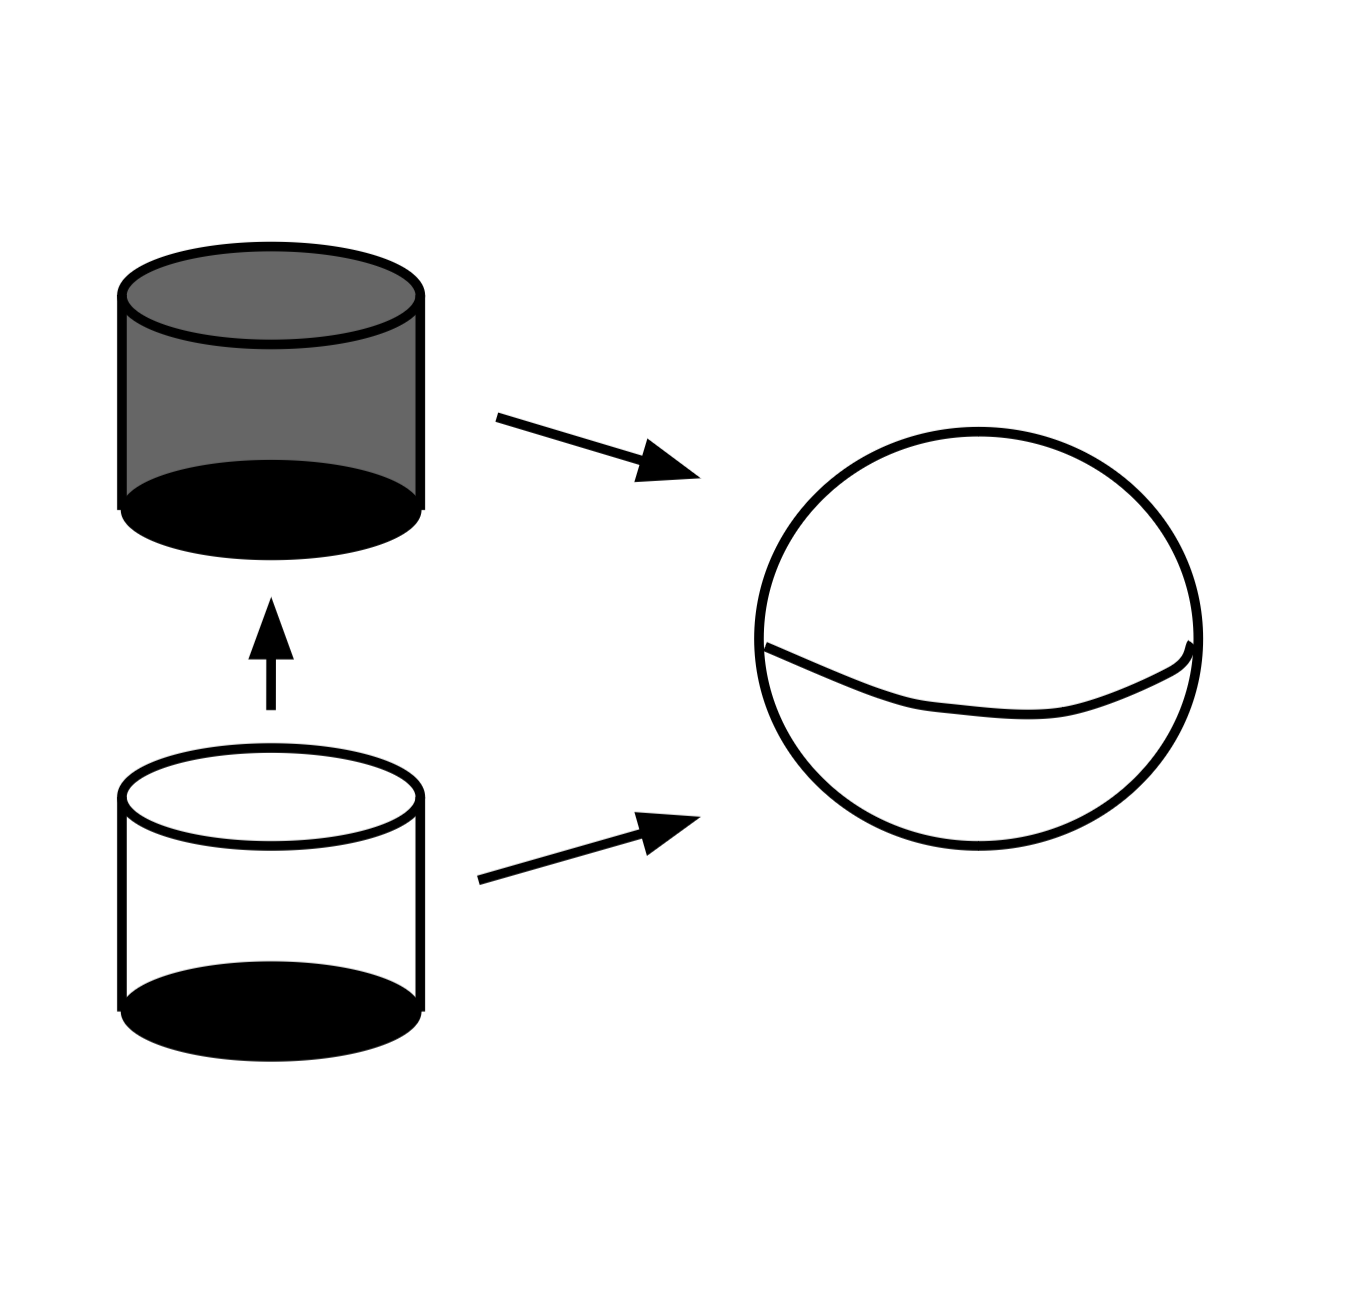
\includegraphics[width=0.5\textwidth]{HEP.png}
\end{center}

{\bf Prism Filling (PF)} Let Y be a quasicategory, and let f, g : ∂Δⁿ ⭢ Y. A homotopy h : ∂Δⁿ × Δ¹ ⭢ Y between f, g : ∂Δⁿ ⭢ Y extends to a map H : Δⁿ × Δ¹ ⭢ Y; this follows from the condition that Y be a quasicategory. H(-,1) and g match on ∂Δⁿ, producing a map f : X ⭢ Y, where X consists of two copies of Δⁿ glued together at the boundary. Consider a space X' formed as a quotient of Δⁿ × Δ¹ by ∂Δⁿ × Δ¹. There is a map φ : X ⭢ X'. An induction hypothesis on f and g involving πₙ ensures that the aparent map X ⭢ Y lifts along φ, producing a map from Δⁿ × Δ¹ which is constant on ∂Δⁿ × Δ¹. Stacking this on top of H can be done using an isomorphism between Δ¹ and Δ¹ glued with itself along different endpoints. Altogether this produces a homotopy between f and g.\\

Directed prism filling may combine fruitfully with the yoneda lemma and/or the fact that simplicial sets are determined by the sets [Δⁿ,X] along with combinatorial information (face and degeneracy maps).

{\bf Decomposing Δⁿ × Δ¹ into a colimit involving n+1 Δ${}^{n+1}$'s} ...

\begin{center}
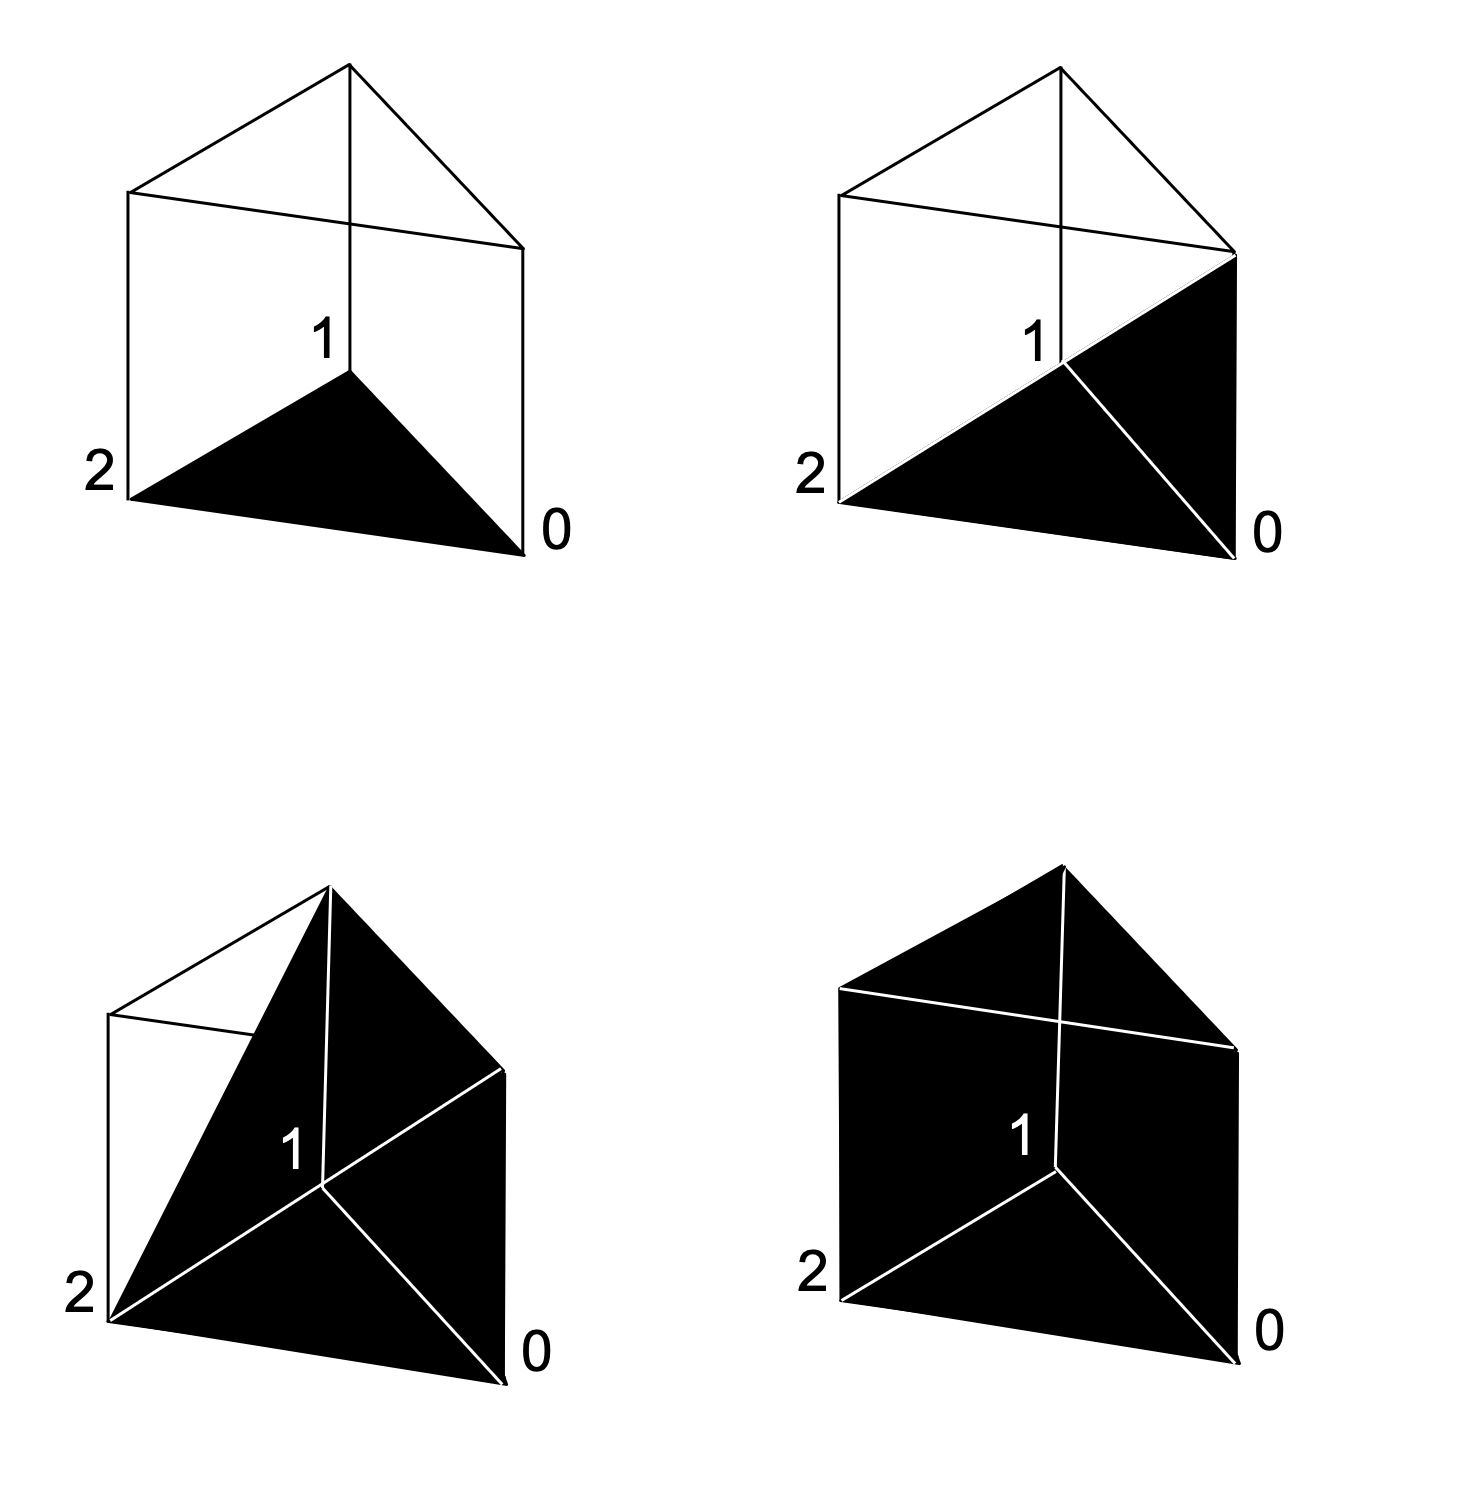
\includegraphics[width=300pt]{prismfilling.png}
\end{center}

In the above, it may be easier if we make use of sub-simplicial sets and prove the theorem using that colimit applied to a natural isomorphism of diagrams products an isomorphism.\\

The decomposition 

A definition of Π⃗ₙ which is consistent with our goals of Wa and Pa is one as a certain pushout involving (Ω⃗ⁿ X)-- one which amounts to taking an equivalence relation by paths in Ω⃗ⁿ X which restrict to constant paths along the face maps fᵢ : Ω⃗${}^{n-1}$ X ⭢ Ω⃗ⁿ X. Here, Ω⃗ is easy to define in the model of quasi-categories, and it amounts . Besides fullfilling our goal of the first Whitehead theorem and puppe sequence, this definition of Π⃗ₙ strikes me as elegant because it uses all of the ways for Ω⃗ⁿ X to map into Ω⃗${}^{n+1}$ X.\\

The next symbols in the project's ``periodic table" that we construct, after Ω⃗ and Π⃗ₙ, will be B⃗ and E⃗, which we feature in the chapter on Puppe sequence (a).\\

A useful thing for us to construct first is the boundary of a product of Δ¹'s and the boundary of a directed simplex. We might even like to expand on this later, but for now just consider for a moment how each might be made out of a glueing construction involving face maps.\\

Even though the Π⃗ₙ's can be defined using Ω⃗ⁿ X and various face maps f$\_(n,b)$ : Ω⃗${}^{n-1}$ X ⭢ Ω⃗${}^{n}$ X for $b : \{ 0, 1 \}$, it may be nice to have this as a result, with the definition one featuring two cubes glued together along their boundary.\\

This means that we want directed box filling in addition to directed prism filling (but which also uses directed prism filling in its proof).

{\bf Box Filling (BF)} Let Y be a quasicategory, and let f, g : ∂Δⁿ ⭢ Y. A homotopy h : ∂Δⁿ × Δ¹ ⭢ Y between f, g : ∂Δⁿ ⭢ Y extends to a map H : Δⁿ × Δ¹ ⭢ Y; this follows from the condition that Y be a quasicategory. H(-,1) and g match on ∂Δⁿ, producing a map f : X ⭢ Y, where X consists of two copies of Δⁿ glued together at the boundary. Consider a space X' formed as a quotient of Δⁿ × Δ¹ by ∂Δⁿ × Δ¹. There is a map φ : X ⭢ X'. An induction hypothesis on f and g involving πₙ ensures that the aparent map X ⭢ Y lifts along φ, producing a map from Δⁿ × Δ¹ which is constant on ∂Δⁿ × Δ¹. Stacking this on top of H can be done using an isomorphism between Δ¹ and Δ¹ glued with itself along different endpoints. Altogether this produces a homotopy between f and g.\\

This goes hand-in-hand with a definition of Π⃗ₙ which suits (I) and (II) in the  to chapter (3). If we make sure to prove lemmas... 

The box filling and prism filling HEPs can be extended to the case of attaching all cells of a particular fixed dimension and as indexed by simplicial set arising from a set (or Lean 4 $\texttt{Type}$). That is, we might like to extend × $()$ (or possibly somehow a $\texttt{Set}$ as well), and that we may find an interest in the following two definitions of Π⃗ₙ, which are designed to fullfill both (I) and (II) in the chapter's .\\

Breaking down BF further can be done conveniently using sub-simplicial sets, just like we used in the proof of prism filling. 

\begin{center}
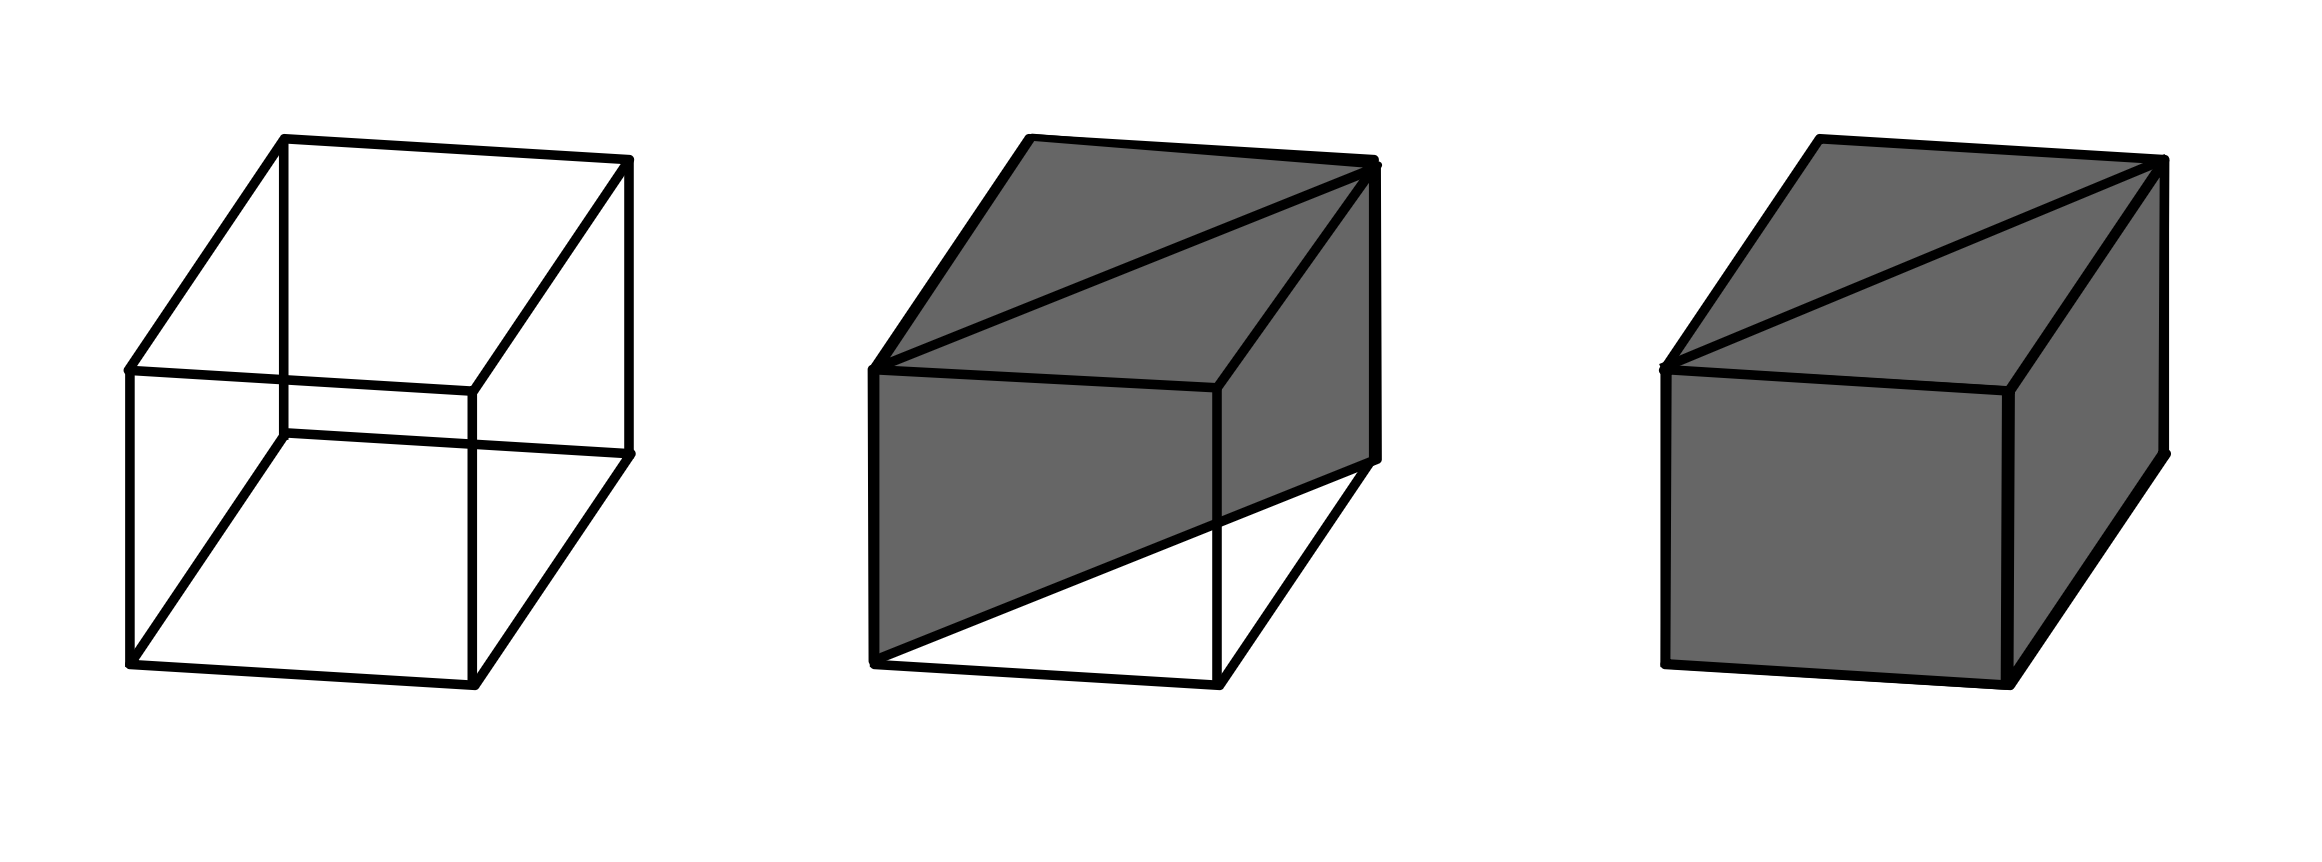
\includegraphics[width=300pt]{boxfilling.png}
\end{center}


{\bf Decomposing (Δ¹)ⁿ into a colimit involving n! Δⁿ's} Consider the face maps fᵢ : Δⁿ ⭢ Δ${}^{n+1}$


The decomposition 
The box filling lemma allows us to prove HEP:


The HEP in the last 

..H(-,1) and g match on ∂Δⁿ, producing a map f : X ⭢ Y, where X consists of two copies of Δⁿ glued together at the boundary. Consider a space X' formed as a quotient of Δⁿ × Δ¹ by ∂Δⁿ × Δ¹. There is a map φ : X ⭢ X'. An induction hypothesis on f and g involving πₙ ensures that the aparent map X ⭢ Y lifts along φ, producing a map from Δⁿ × Δ¹ which is constant on ∂Δⁿ × Δ¹. Stacking this on top of H can be done using an isomorphism between Δ¹ and Δ¹ glued with itself along different endpoints. Altogether this produces a homotopy between f and g.\\

Imagine ...
\fi


\newpage
{
\Huge 
\begin{center}
\ \\
\ \\
\texttt{THE WHITEHEAD THEOREM FOR A}${}^{\infty}$ \texttt{BASED CW-COMPLEXES}
\ \\
\ \\
\end{center}
\thispagestyle{empty}
}

\iffalse

In this first section we prove the standard Whitehead theorem.\\



The proof of the Whitehead theorem divides into REP (replacement for Based ∞-groupoids X : ∞-Grpd₀) and HEP (the homotopy extension property for weak equivalent maps of Based ∞-groupoids). The replacement functor ∞$\texttt{-Grpd}$₀ can be constructed using globular sets.\\

Globular sets are not a rich enough invariant for homotopy, but maps of globular sets bear a criticall difference because of 

\begin{center}
\texttt{∀(E:D(∞-Grpd₀)),∀(B:D(∞-Grpd₀)),∀(f:E ⭢ B),∀(G:E ⭢ B),(∀(n:Nat),(πₙ F = πₙ G)) ⭢ F = G}
\end{center}

\subsection{Globular Sets}

The globe category 𝔾 is the category

\begin{center}
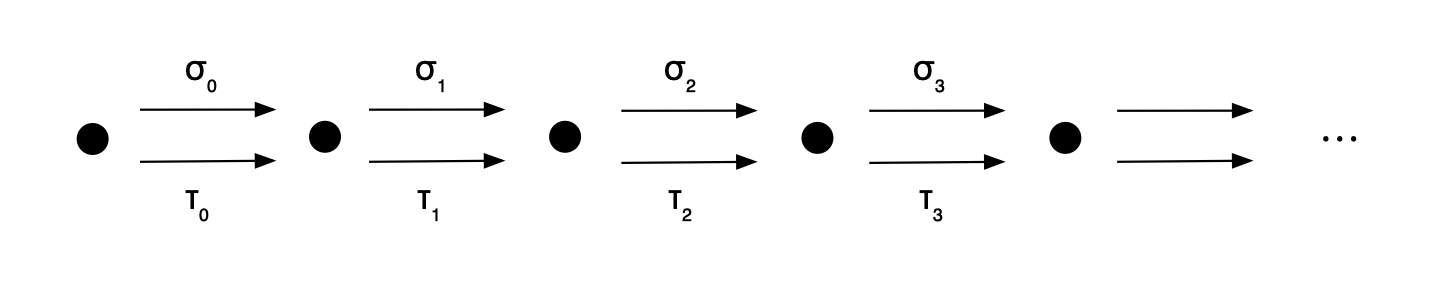
\includegraphics[scale=0.5]{globecat.png}
\end{center}

\href{https://ncatlab.org/nlab/show/globular+set}{Globular sets} are functors from the opposite category of the globe category 𝔾 into the category of sets, and maps of globular sets are natural transformations between them.\\

In this chapter we prove the following (which we have called Whitehead Theorem (c)): ∀(E:D(∞-Grpd₀)),∀(B:D(∞-Grpd₀)),∀(f:E ⭢ B),∀(G:E ⭢ B),(∀(n:Nat),(πₙ F = πₙ G)) ⭢ F = G, where πₙ is notation for π n.\\

This can be shown using CW-replacement and induction on n. Fibrant replacement of an object X entails replacing an object in ∞-Grpd₀ with a CW-object (an object made by successively glueing in higher and higher simplices along their boundaries obtaining a sequence Xₙ). Given an equality π${}_{n+1}(f) = $π${}_{n+1}(g)$ and a homotopy equivalence hₙ : Δ¹ × Xₙ ⭢ Y between $f|_{X_n}, g|_{X_n}$ : Xₙ ⭢ Y, we construct an extension of the homotopy equivalence Δ¹ × $X_{n+1}$ ⭢ Y.\\

\iffalse
Can the attaching map be 
\fi

{\bf Spheres and balls} Next we turn to defining spheres and balls:

{
\footnotesize
\begin{center}
\begin{tabular}{||l || l || l ||} 
 \hline
  & \multicolumn{2}{||c||}{\texttt{Spheres and Balls}} \\
 \hline
 Name of the $\texttt{X}$ value & \texttt{∂X ≅ Sⁿ} & \texttt{X ≅ Dⁿ} \\
 \hline
 \hline
 p-norm unit ball for p = 1 & ∂B(1,1) & B(1,1) \\
 \hline
 p-norm unit ball for 1 < p < 2 & ∂B(p,1) & B(p,1) \\
 \hline
 p-norm unit ball for p = 2 & ∂B(2,1) & B(2,1) \\
 \hline
 p-norm unit ball for 2 < p < ∞ & ∂B(p,1) & B(p,1) \\
 \hline
 p-norm unit ball for p = ∞ & ∂B(∞,1) & B(∞,1) \\
 \hline
 The n-simplex & ∂Δⁿ & Δⁿ \\
 \hline
 \hline
\end{tabular}
\end{center}
}

\begin{definition}
...
\end{definition}

\iffalse
\begin{definition}
Define a function d${}^{(n_1,...,n_k)} : $ D${}^{n_1}$ × $\cdots$ × D${}^{n_k}$ ⭢ D${}^{n_1 + \cdots + n_k}$ sending $(x_1,...,x_k)$...
\end{definition}
\fi

\begin{theorem}
i¹ : S⁰ ⭢ D¹ 
\end{theorem}

\begin{theorem}
Dⁿ × D¹ ⭢ Dⁿ⁺¹
\end{theorem}

\begin{definition}
Dⁿ ⭢ Dᵐ
\end{definition}


\begin{theorem}
Fix n : ℕ and let ∂ⁿ : Sⁿ ⭢ Dⁿ⁺¹ be the inclusion. The pushout of the following diagram is isomorphic to Sⁿ⁺¹:
\begin{center}
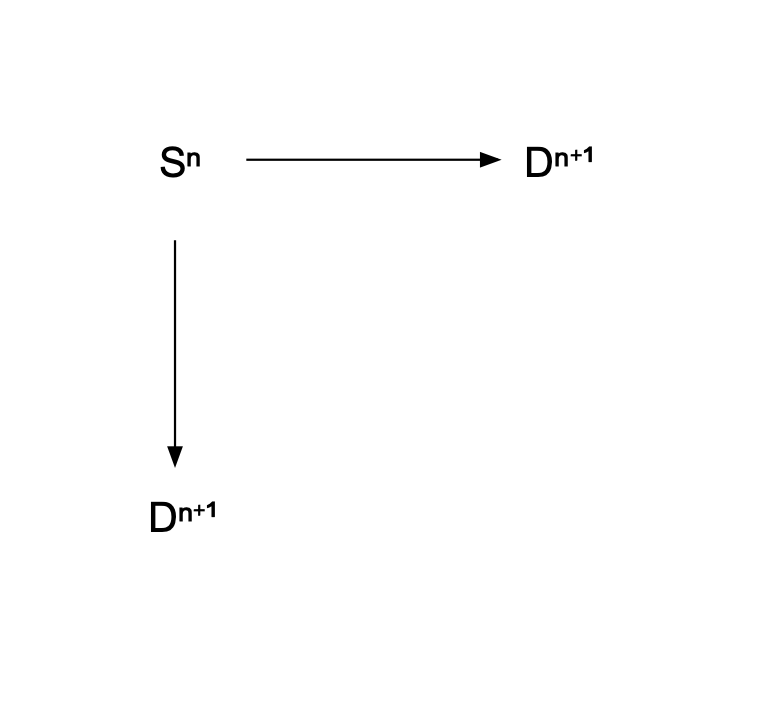
\includegraphics[scale=0.5]{pushout.png}
\end{center}
\end{theorem}

\begin{proof}

\end{proof}


\begin{theorem}
Define a function ||-||${}_{2}$ : Dⁿ ⭢ I sending (x₁,...,xₙ) to $\sqrt{\sum_{i = 1}^n x_i^2}$, and write ||-||${}_{2}$
\end{theorem}

\begin{proof}
...
\end{proof}

\subsection{HEP for Based ∞-groupoids}

In this section we prove the homotopy extension property for Based ∞-groupoids, which we here model as CW-complexes.\\


{\bf Jar filling} Next we turn to defining `jar shapes' $\texttt{Jⁿ}$, which include into $\texttt{Dⁿ × I}$ $\texttt{iₙ : Jⁿ ⭢ Dⁿ × I}$, after which we `fill' them (i.e. demonstrate that any continuous map f : Jⁿ ⭢ X extends to a continuous map g : Dⁿ × I ⭢ X).\\

The first and most common approach involves `shining a light ray down from above the jar', i.e. projection. We obtain a formula for .\\

The second way to fill the jar




{\bf Change of Base} Jar filling leaves the question

\begin{definition}
Let X₋₁ be a connected CW-complex and let n : Nat be a natural number. The transport function $\texttt{trans\ n\ X₋₁ : (f : [I,X₋₁])  → πₙ (f 0) ⭢ πₙ (f 1)}$ is 
\end{definition}

\begin{theorem}
Let X₋₁ be a connected CW-complex and let f : I ⭢ X₋₁ be a path, so that $\texttt{(trans\ n X₋₁ f⁻¹) • (trans\ n X₋₁ f)}$ has type $\texttt{πₙ (f 0) ⭢ πₙ (f 0)}$. Then
\begin{center}
$\texttt{(trans\ n X₋₁ f⁻¹) • (trans\ n X₋₁ f) = 1\_(πₙ (f 0))}$
\end{center}
\end{theorem}

\begin{proof}
...
\end{proof}

The proof in the above can be depicted like so, as a `painting with two concentric frames':

\iffalse
\begin{center}
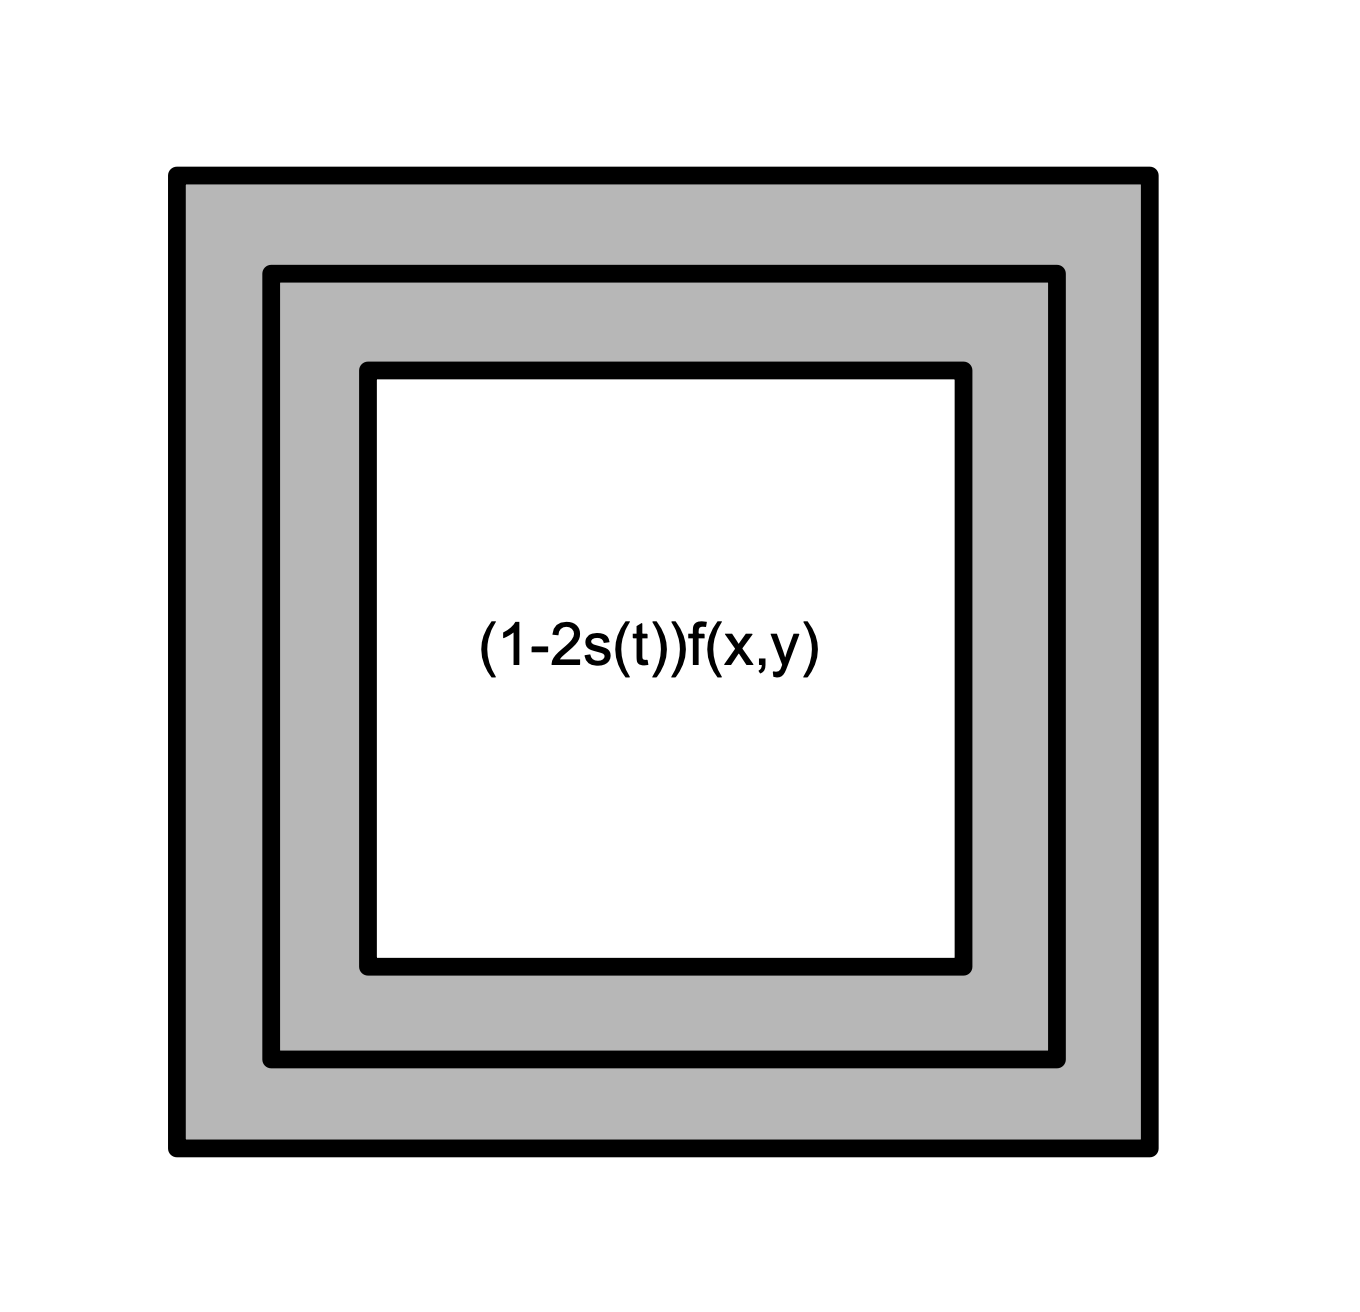
\includegraphics[scale=0.5]{pictureframe.png}
\end{center}
\fi


that the Based CW-complexes (X₋₁,x) and (X₋₁,y) are 

\begin{theorem}

\end{theorem}

\begin{proof}
...
\end{proof}

\begin{center}
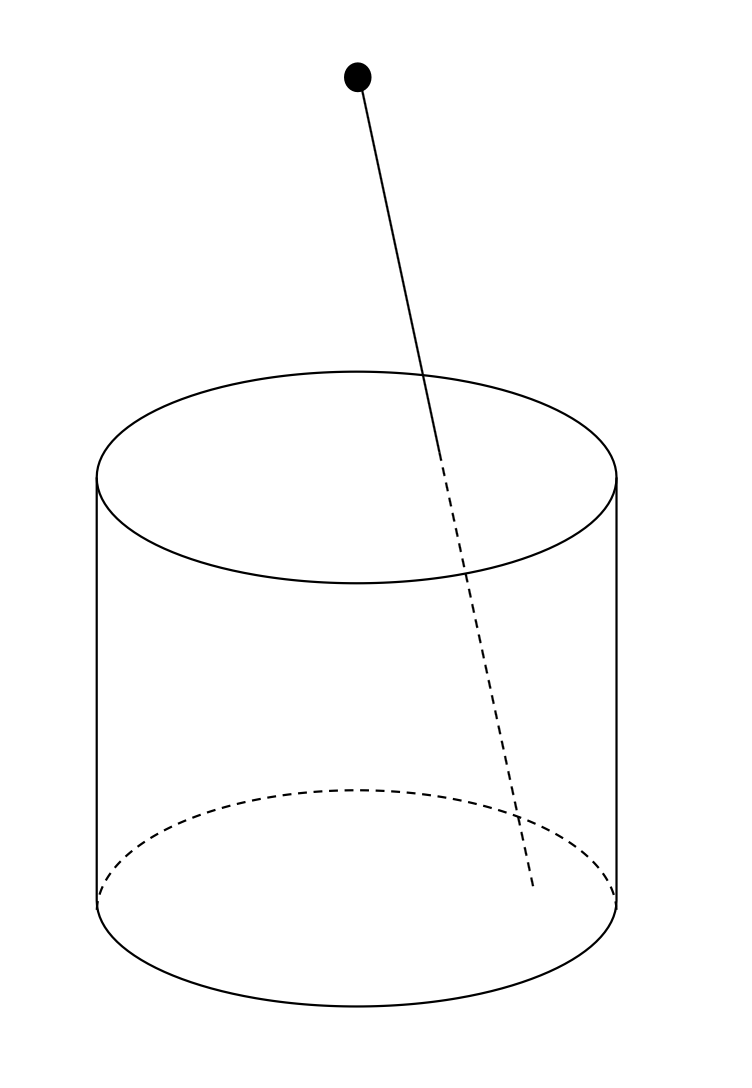
\includegraphics[width=3.5cm,height=5cm]{proj.png}
\end{center}


\subsection{REP for Based ??? ∞-categories}

In this section we use the notion of globular sets to replace a topological space with a CW-complex. Together with HEP (homotopy extension), this will complete the proof of the Whitehead theorem.




\fi


\newpage
{
\Huge 
\begin{center}
\ \\
\ \\
\texttt{THE WHITEHEAD THEOREM}\\
\texttt{FOR A}${}^{\infty}$ $\infty$\texttt{-CATEGORIES}
\ \\
\ \\
\end{center}
\thispagestyle{empty}
}

\iffalse
\section{Chapter 13: ∞\texttt{-Cat}}

This chapter and the next chapter are more technical and difficult than the rest of the book.\\

\begin{enumerate}
\item Defining D(∞-Cat) by formally inverting weak equivalences.
\item Defining D(∞-Cat/C) by formally inverting weak equivalences.
\item Defining a fibrant replacement functor for ∞-Cat
\item Defining a fibrant replacement functor for ∞-Cat/C
\item We first construct both the category D(∞-Cat) and, for each C : D(∞-Cat), the category D(∞-Cat/C) by formally inverting weak equivalences in the category of quasicategories and the category of quasicategories over C.
\end{enumerate}

\subsection{Ω⃗}

Our choice of symbols refects our choice of three variations of the Whitehead theorem and three Puppe sequences. Ω⃗, the analogue of loop space, is the internal hom functor [Δ¹,-] : ∞-Cat ⭢ ∞-Cat. This is not hard to construct, with the main lemma being that the path space of a quasicategory has the quasicategory lifting conditon.\\

We will be interested in one formal model of D(∞-Cat) which consists of formal compositions f₁ • g₁ • f₂ • g₂ • ⋯ • fₙ • gₙ, where gₙ $: Dom(f{}_{n+1}) $⭢ ??? is a weak equivalence, and something similar for D(∞-Cat). However, it is still vital to have the replacement functor $\texttt{repl}$, which ensures the Whitehead theorem for particular ∞-categories which are constructed out of attaching maps.\\


\subsection{ω⃗}

Ω⃗ is to internal categories as ω⃗ is to internal C-presheaves. It is also called directed homotopy pullback. These functors will later be used to produce functors P⃗ : D(∞-Cat) ⭢ InternalCategory D(∞-Cat) and p⃗ : D(∞-Cat⁄C) ⭢ InternalPresheaf (P⃗ C) D(∞-Cat⁄C).\\


\subsection{Π⃗ₙ}

The mentioned functors Π⃗ₙ are designed with both Whitehead theorem (a) and Puppe sequence (a) in mind.



\section{Chapter 14: The Whitehead Theorem for ∞-Categories}

\iffalse
https://mathoverflow.net/questions/368596/intuition-for-categorical-fibrations#:~:text=a%20left%2Fright%20fibration%20is,categories%20with%20correspondences%20between%20fibers.
\fi


\subsection{Directed Cubical Complexes}

...\\


In this chapter, we take on the objective of Whitehead theorem (a), out of which we will prove the other more concrete Whitehead theorems:\\

\begin{center} ∀(E:D(∞-Cat)),∀(B:D(∞-Cat)),∀(F:E ⭢ B),∀(G:E ⭢ B),(∀(n:Nat),(Π⃗ₙ F = Π⃗ₙ G)) ⭢ F = G
\end{center}

We can attempt to form a slightly different category, much like the above, called 𝓓(∞-Cat), at first, and in a formal way, so as to create a category whose object component 𝓓(∞-Cat).α matches the object component ∞-Cat.α while featuring the above theorem in a formal way. However, with this as our model of D(∞-Cat), we may then also be interested in the establishment of a model in which the Whitehead theorem is demonstrated, with the main idea being to prove two complementary concepts:

\begin{enumerate}
\item (REP) Establish a kind of ``weak equivalent fibrant replacement" R : ∞-Cat.α ⭢ ∞-Cat.α (.α gives the object component in Mathlib's category theory library), analogous to CW-complex replacement in Whitehead's original paper. It's especially nice if R forms the object component of a functor F : ∞-Cat ⭢ ∞-Cat. D(F) : D(∞-Cat) ⭢ D(∞-Cat) should be a categorical equivalence, and that is what we will do.
\item (HEP) For the object R X, demonstrate that any F,G : (R X) ⭢ Y such that ∀(n:Nat),(Π⃗ₙ F = Π⃗ₙ G), there is a directed homotopy equivalence between F and G. Note that ``directed homotopy equivalence" consists of a composible sequence of simple directed homotopies Hᵢ : Δ¹ × (R X) ⭢ Y, 1 ≤ i ≤ n, with even Hᵢ running reverse to the odd Hᵢ.
\end{enumerate} 

Both of these will use induction on Lean's $\texttt{Nat}$. The first of these could be called a REP (for REplacement Property, but this isn't usual terminology), and the second typically uses induction and a HEP (Homotopy Extension Property). Our REPa will consist of objects made out of particular kinds of pushouts called attaching maps, and can be made functorial. Proving the HEPa can be done by well-order induction on the attaching maps present in our choice of R, thereby reducing to the case of extending a homotopy along a single attachment.\\

Our HEPa (directed box filling) is similar to the HEP shown in Whitehead's original paper, and to the approach detailed in Hatcher's textbook, though no doubt modified to suit our two goals:

\begin{enumerate}[(I)]
\item The analogue of the Puppe sequence on the front cover needs to hold.
\item The first Whitehead theorem on the front cover needs to hold.
\end{enumerate}

These two considerations determine our choice of Π⃗ₙ, Ω⃗, and ω⃗. We take Ω⃗ to be (simply) the internal hom functor [Δ¹,-] (which requires showing that Ω⃗X has the inner-horn filling condition). ω⃗ is then defined as a certain pullback of Ω⃗, and Π⃗ₙ is designed to produce a Puppe sequence with a meaningful notion of exactness by which we can demonstrate the goal of recognition theorems (i) and (ii). Specifically, it makes sense to use cubes in our definition of Π⃗ₙ because of how they are representing objects of Ω⃗ⁿ. Meanwhile, it is also clear that the quotient producing Π⃗ₙ is subtle in exactly how it requires fixing the endpoints of a sequence of alternating directed homotopies. We will define Π⃗ₙ's by identifying those objects x, y: Ω⃗ⁿ X which are homotopic by a homotopy which restricts to a constant along the face maps fᵢ : Ω⃗${}^{n-1}$ X ⭢ Ω⃗${}^{n-1}$ X (which correspond to Maps (n,b), where b : Bool).\\

Imagine for a moment the picture of a square shaped cusion; we might make such a cusion by first soeing together 6 squares of cloth and filling it with material, then "soeing the walls down to a square". Here we go with this:

\begin{enumerate}
\item Define a n-cubical cusion using the boundary of an n-1 cube times Δ¹, i.e. the quotient of (Δ¹)${}^{n-1}$ × Δ¹ by an equivalence relation, but we have to start our model somewhere), or perhaps more easily the pushout of f : Δ¹ × (∂((Δ¹)ⁿ)) ⭢ (Δ¹)${}^{n+1}$ by the projection map Δ¹ × (∂((Δ¹)ⁿ)) ⭢ ∂((Δ¹)ⁿ)
\item Define a simplicial cusion using the boundary of an n-1 simplex times Δ¹, i.e. the quotient of (Δ¹) by an equivalence relation, or perhaps more easily the pushout of f : Δ¹ × (∂(Δⁿ)) ⭢ (Δ¹) × Δⁿ by the projection map Δ¹ × (∂((Δ¹)ⁿ)) ⭢ ∂(Δⁿ)
\end{enumerate}

The boundary of a cusion is a pouch, isomorphic to a pushout of two cubes glued together at their boundaries:

\begin{enumerate}
\item Define a n-cubical pouch as the pushout of two boundary maps ∂((Δ¹)ⁿ) ⭢ (Δ¹)ⁿ
\item Define a simplicial pouch as the pushout of two boundary maps ∂(Δⁿ) ⭢ Δⁿ
\end{enumerate}

Notice that paths in Ω⃗ⁿX produce paths in Ω⃗${}^{n-1}$X in as many ways as there are face maps (Δ¹)${}^{n-1}$ ⭢ Δ¹${}^{n}$, these could be called restrictions and are no doubt related to the pouches and cusions we just defined. The cartesian closed structure on simplicial sets with the lifting condition clarifies the relationship between the two available definitions of Π⃗ₙ:

\begin{enumerate}
\item Homotopies of maps from a cube which are constant on the boundary
\item Paths of maps in Ω⃗${}^{n-1}$X which produce constant maps under the mentioned restritions.
\item Maps from a pouch mod an equivalence relation (really we phrase this as a pushout!), namely the equivalence relation in which any two maps from a pouch that extend to maps from a cusion are identified.
\end{enumerate}

After we construct Π⃗ₙ in the first section, we will be in a place to demonstrate that the natural transformation $\texttt{weak\_equivalence : repl ⭢ (𝟙 }$∞$\texttt{-Cat)}$ consists of weak equivalences (a fact which we call REP, which is short for REplacement Principal). This is covered in the section titled REP, which also constructs $\texttt{repl}$ and $\texttt{weak\_requivalence}$.\\

In sum, the goal of the present chapter is to use similar insights to the proof of the Whitehead theorem featured Hatcher's textbook to prove Wa and Pa for the model of quasicategories, using Mathlib's predefined horns and simplices in its simplicial sets section. The main difference is that our work must take care to respect the directed nature of quasicategories.\\

\iffalse
In the future, we intend to add important aspects of the bigger picture besides those which directly establish REP and HEP in the sections below. These are important considerations in ensuring usability. Three different model structures on ∞-Cat ensue from the six definitions below, which are contained in Lurie's ``Higher Topos Theory" on page 53, and which are due to Joyal:

\begin{definition} A morphism $\texttt{f : X ⭢ S}$ of simplicial sets is
\begin{enumerate}
\item A left fibration if f has the right lifting property with respect to all
horn inclusions Λni ⊆ ∆n, 0 ≤ i < n.
\item A right fibration if f has the right lifting property with respect to all
horn inclusions Λni ⊆ ∆n, 0 < i ≤ n.
\item An inner fibration if f has the right lifting property with respect to all
horn inclusions Λni ⊆ ∆n, 0 < i < n.
\end{enumerate}
A morphism of simplicial sets $\texttt{i : A ⭢ B}$ is
\begin{enumerate}
\item left anodyne if $\texttt{i}$ has the left lifting property with respect to all left fibrations.
\item right anodyne if $\texttt{i}$ has the left lifting property with respect to all right fibrations.
\item inner anodyne if $\texttt{i}$ has the left lifting property with respect to all inner fibrations.
\end{enumerate}
\end{definition}
\fi

\begin{enumerate}
\item Defining $\texttt{repl}$
\item 
\end{enumerate}

\section{REP}

We have divided the work of proving Whitehead theorem (a) into two steps: REP and HEP. In this section, we construct a functor $\texttt{repl : }$∞$\texttt{-Cat ⭢ }$∞$\texttt{-Cat}$ along with a natural transformation $\texttt{weak\_equivalence : repl ⭢ (𝟙 }$∞$\texttt{-Cat)}$. To construct $\texttt{repl}$ 


\section{HEP}

Consider the context of , supposing that we have constructed a homotopy ... This gives a picture that is a bit like ``filling up a jar``: a homotopy h : of f, g : ∂Δ² ⭢ Y, along with the value of g on Δ², produces a ``jar" shape in Y, which can be ``filled up" to produce a homotopy h : Δ¹ × Δ² ⭢ Y. This is easier for simplicial-Based approaches than for point-set topological approaches, the latter of which needs extra steps that deform a map into a cellular map.\\

This construction, in the case of point set topology, often involves first deforming maps so as to be cellular; however our analogue of CW complexes allows us to skip this step.\\

This construction (HEP for quasicategories) may even be equivalent to the quasicategory lifting condition if we are lucky. It is also the main technical device allowing for our concrete choice of model (quasicategories).\\

In this section, we demonstrate this extension property and use it to conclude the Whitehead theorem for ∞-categories stated above.\\

\begin{center}
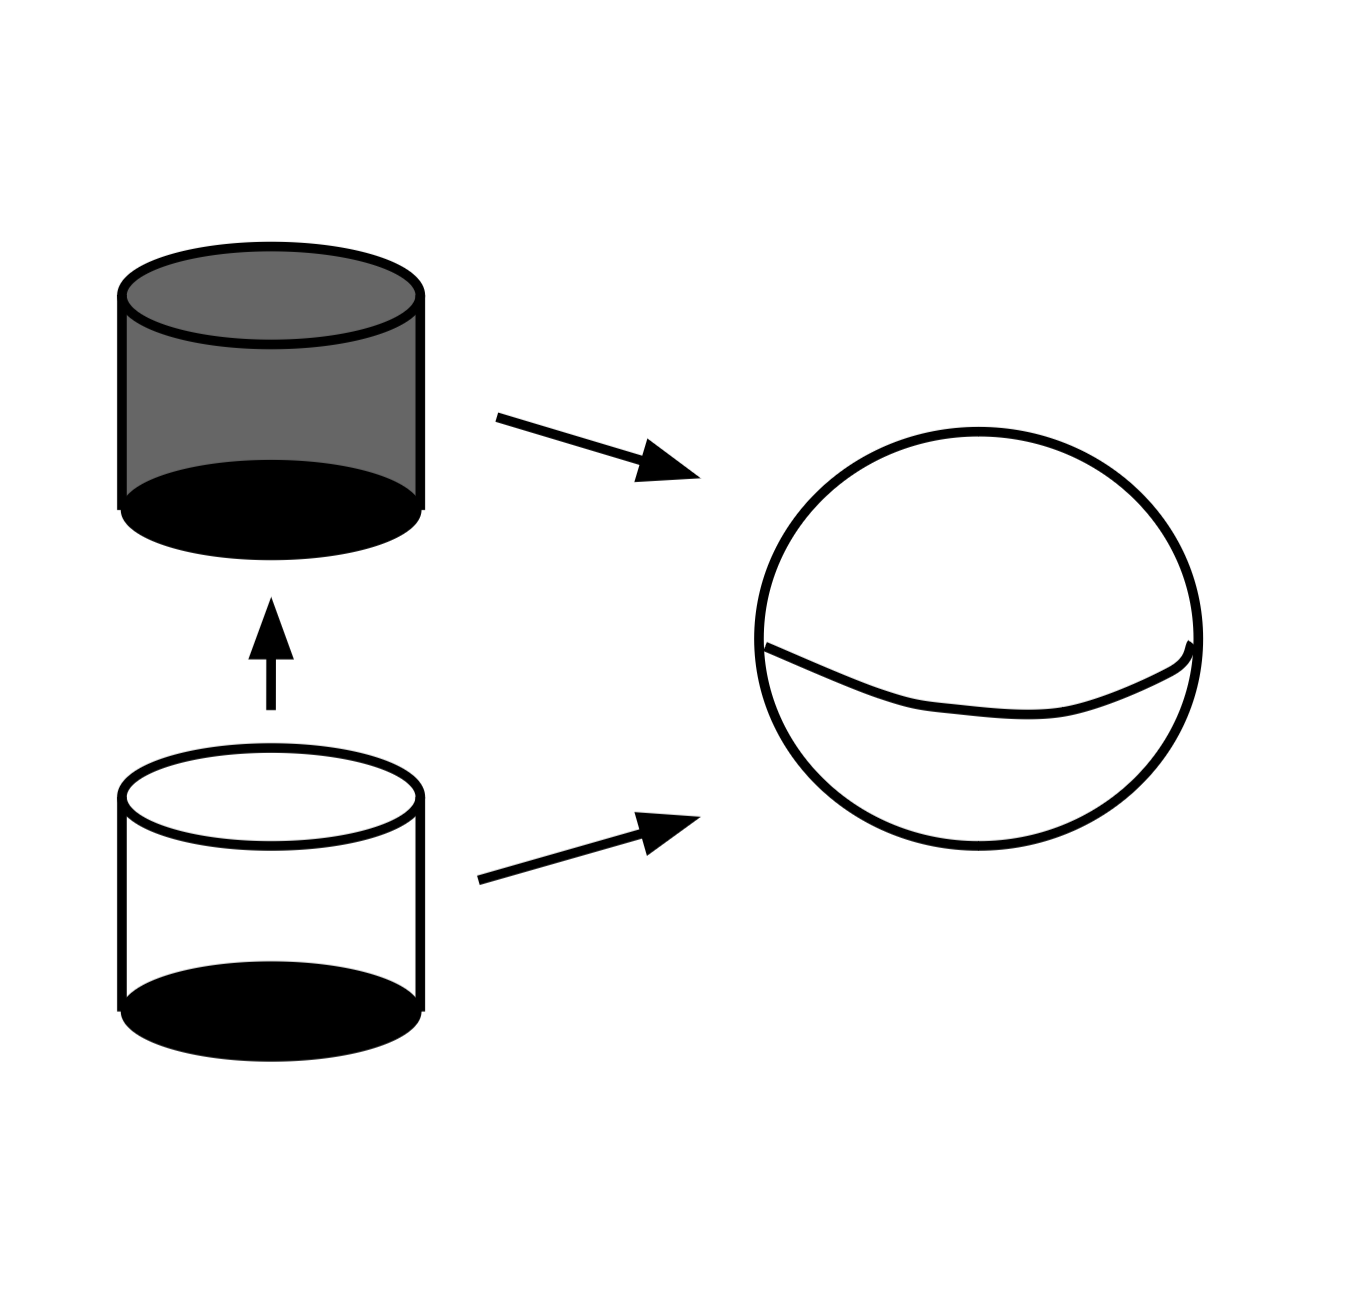
\includegraphics[width=0.5\textwidth]{HEP.png}
\end{center}

{\bf Prism Filling (PF)} Let Y be a quasicategory, and let f, g : ∂Δⁿ ⭢ Y. A homotopy h : ∂Δⁿ × Δ¹ ⭢ Y between f, g : ∂Δⁿ ⭢ Y extends to a map H : Δⁿ × Δ¹ ⭢ Y; this follows from the condition that Y be a quasicategory. H(-,1) and g match on ∂Δⁿ, producing a map f : X ⭢ Y, where X consists of two copies of Δⁿ glued together at the boundary. Consider a space X' formed as a quotient of Δⁿ × Δ¹ by ∂Δⁿ × Δ¹. There is a map φ : X ⭢ X'. An induction hypothesis on f and g involving πₙ ensures that the aparent map X ⭢ Y lifts along φ, producing a map from Δⁿ × Δ¹ which is constant on ∂Δⁿ × Δ¹. Stacking this on top of H can be done using an isomorphism between Δ¹ and Δ¹ glued with itself along different endpoints. Altogether this produces a homotopy between f and g.\\

Directed prism filling may combine fruitfully with the yoneda lemma and/or the fact that simplicial sets are determined by the sets [Δⁿ,X] along with combinatorial information (face and degeneracy maps).

{\bf Decomposing Δⁿ × Δ¹ into a colimit involving n+1 Δ${}^{n+1}$'s} ...

\begin{center}
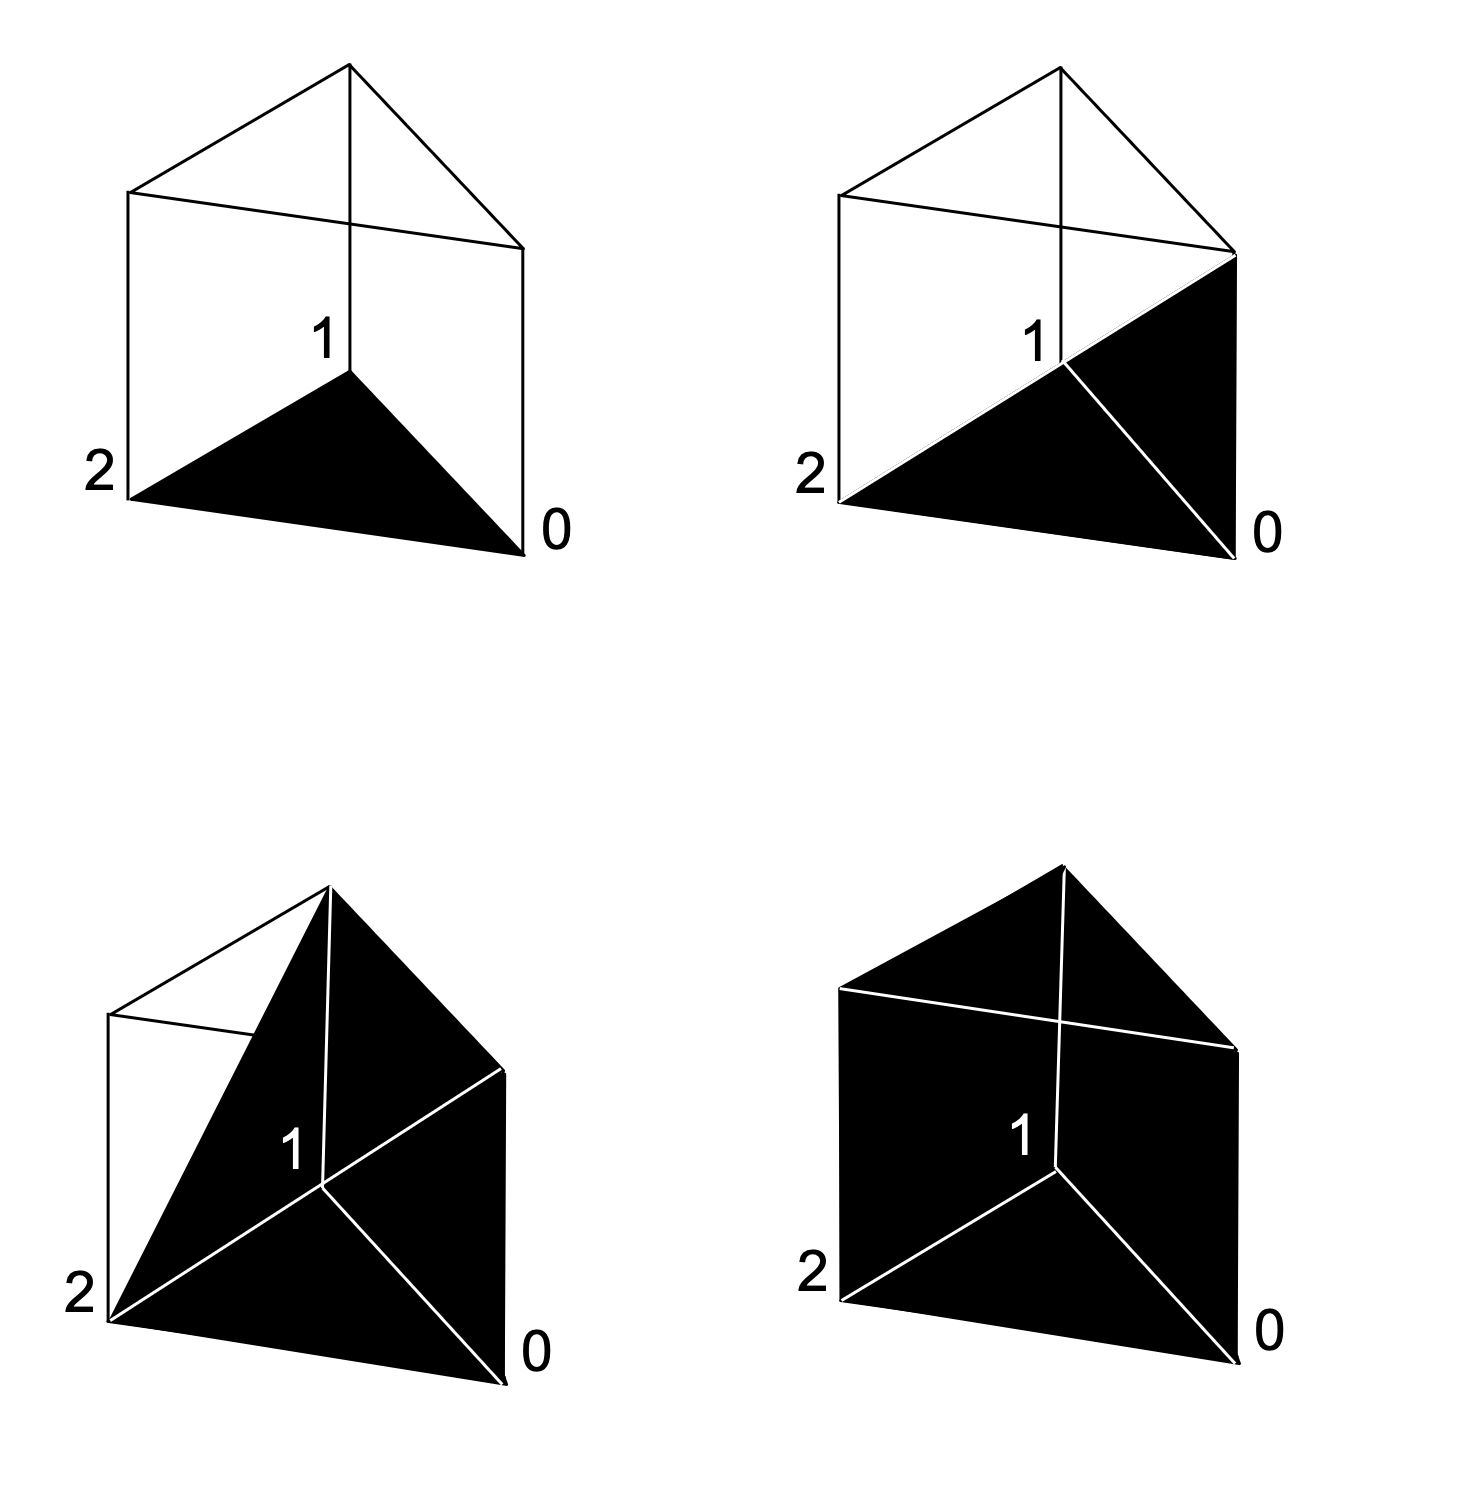
\includegraphics[width=300pt]{prismfilling.png}
\end{center}

In the above, it may be easier if we make use of sub-simplicial sets and prove the theorem using that colimit applied to a natural isomorphism of diagrams products an isomorphism.\\

The decomposition 

A definition of Π⃗ₙ which is consistent with our goals of Wa and Pa is one as a certain pushout involving (Ω⃗ⁿ X)-- one which amounts to taking an equivalence relation by paths in Ω⃗ⁿ X which restrict to constant paths along the face maps fᵢ : Ω⃗${}^{n-1}$ X ⭢ Ω⃗ⁿ X. Here, Ω⃗ is easy to define in the model of quasi-categories, and it amounts . Besides fullfilling our goal of the first Whitehead theorem and puppe sequence, this definition of Π⃗ₙ strikes me as elegant because it uses all of the ways for Ω⃗ⁿ X to map into Ω⃗${}^{n+1}$ X.\\

The next symbols in the project's ``periodic table" that we construct, after Ω⃗ and Π⃗ₙ, will be B⃗ and E⃗, which we feature in the chapter on Puppe sequence (a).\\

A useful thing for us to construct first is the boundary of a product of Δ¹'s and the boundary of a directed simplex. We might even like to expand on this later, but for now just consider for a moment how each might be made out of a glueing construction involving face maps.\\

Even though the Π⃗ₙ's can be defined using Ω⃗ⁿ X and various face maps f$\_(n,b)$ : Ω⃗${}^{n-1}$ X ⭢ Ω⃗${}^{n}$ X for $b : \{ 0, 1 \}$, it may be nice to have this as a result, with the definition one featuring two cubes glued together along their boundary.\\

This means that we want directed box filling in addition to directed prism filling (but which also uses directed prism filling in its proof).

{\bf Box Filling (BF)} Let Y be a quasicategory, and let f, g : ∂Δⁿ ⭢ Y. A homotopy h : ∂Δⁿ × Δ¹ ⭢ Y between f, g : ∂Δⁿ ⭢ Y extends to a map H : Δⁿ × Δ¹ ⭢ Y; this follows from the condition that Y be a quasicategory. H(-,1) and g match on ∂Δⁿ, producing a map f : X ⭢ Y, where X consists of two copies of Δⁿ glued together at the boundary. Consider a space X' formed as a quotient of Δⁿ × Δ¹ by ∂Δⁿ × Δ¹. There is a map φ : X ⭢ X'. An induction hypothesis on f and g involving πₙ ensures that the aparent map X ⭢ Y lifts along φ, producing a map from Δⁿ × Δ¹ which is constant on ∂Δⁿ × Δ¹. Stacking this on top of H can be done using an isomorphism between Δ¹ and Δ¹ glued with itself along different endpoints. Altogether this produces a homotopy between f and g.\\

This goes hand-in-hand with a definition of Π⃗ₙ which suits (I) and (II) in the  to chapter (3). If we make sure to prove lemmas... 

The box filling and prism filling HEPs can be extended to the case of attaching all cells of a particular fixed dimension and as indexed by simplicial set arising from a set (or Lean 4 $\texttt{Type}$). That is, we might like to extend × $()$ (or possibly somehow a $\texttt{Set}$ as well), and that we may find an interest in the following two definitions of Π⃗ₙ, which are designed to fullfill both (I) and (II) in the chapter's .\\

Breaking down BF further can be done conveniently using sub-simplicial sets, just like we used in the proof of prism filling. 

\begin{center}
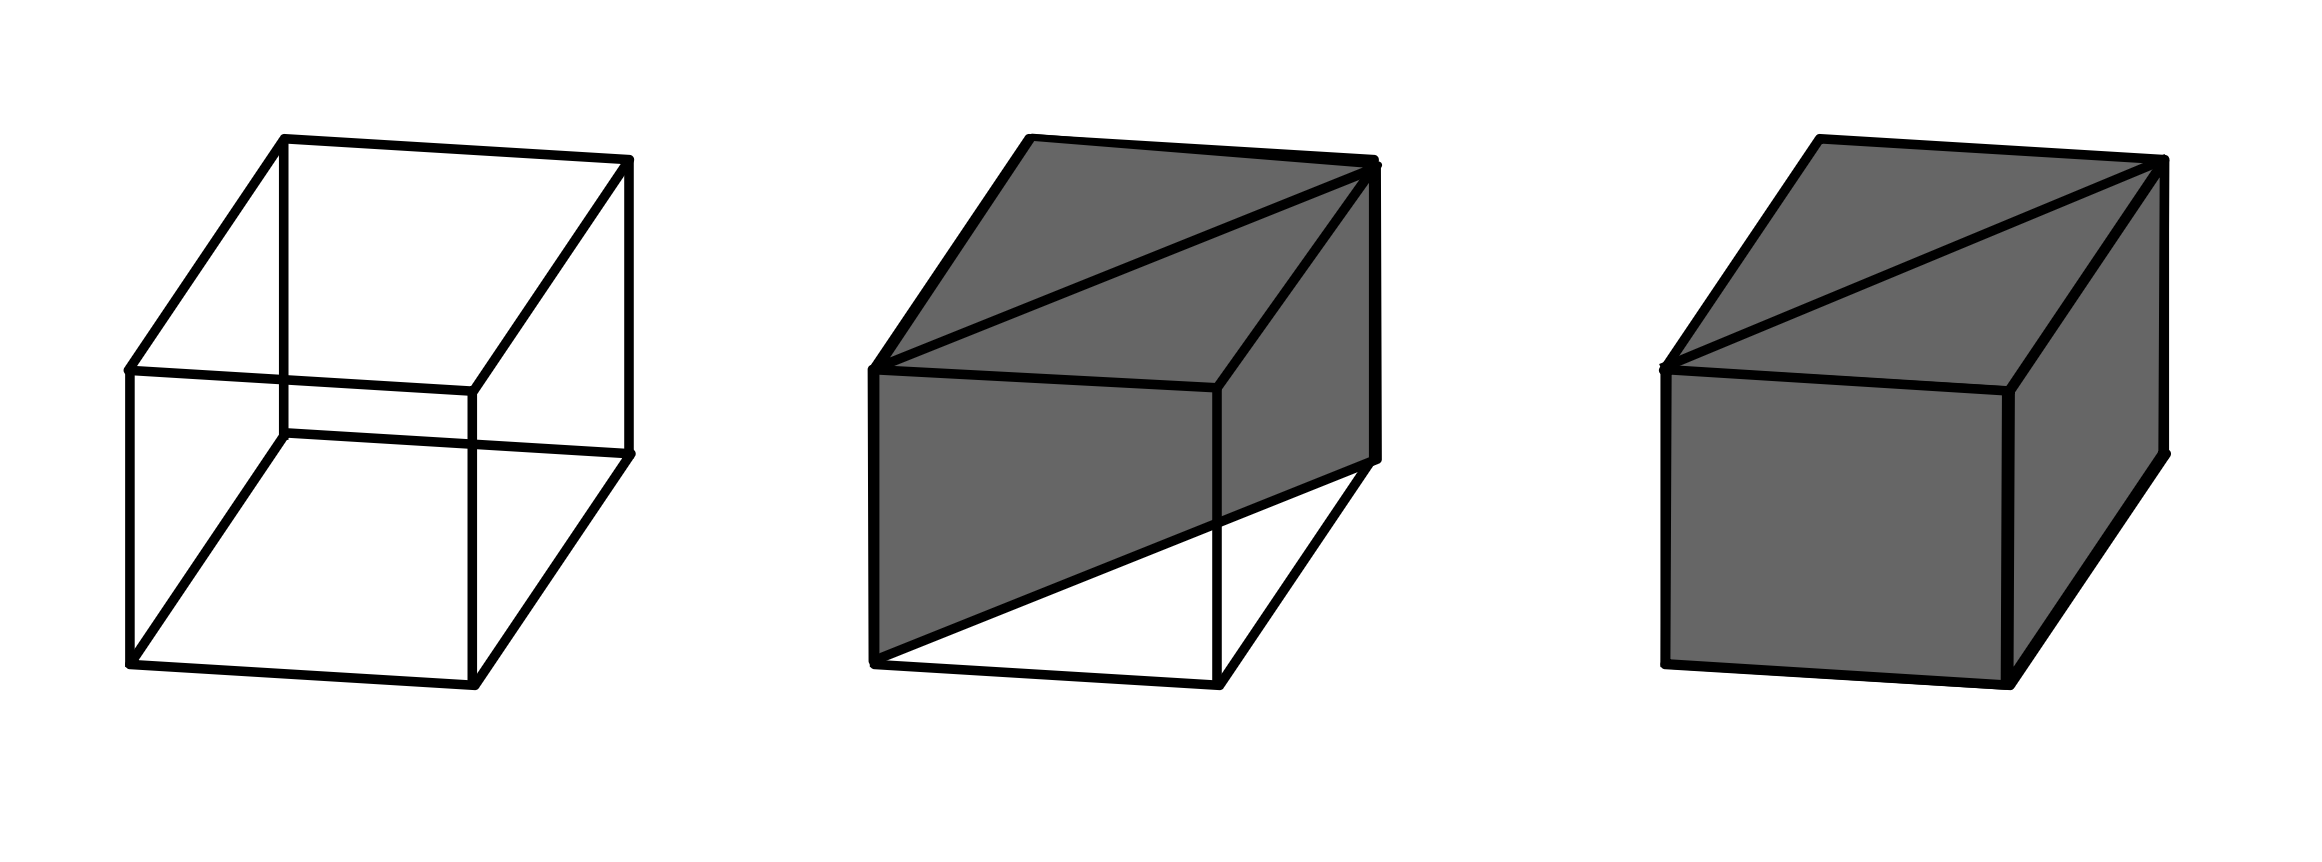
\includegraphics[width=300pt]{boxfilling.png}
\end{center}


{\bf Decomposing (Δ¹)ⁿ into a colimit involving n! Δⁿ's} Consider the face maps fᵢ : Δⁿ ⭢ Δ${}^{n+1}$


The decomposition 
The box filling lemma allows us to prove HEP:


\section{The Whitehead Theorem for ∞-Cat}

The HEP in the last 

..H(-,1) and g match on ∂Δⁿ, producing a map f : X ⭢ Y, where X consists of two copies of Δⁿ glued together at the boundary. Consider a space X' formed as a quotient of Δⁿ × Δ¹ by ∂Δⁿ × Δ¹. There is a map φ : X ⭢ X'. An induction hypothesis on f and g involving πₙ ensures that the aparent map X ⭢ Y lifts along φ, producing a map from Δⁿ × Δ¹ which is constant on ∂Δⁿ × Δ¹. Stacking this on top of H can be done using an isomorphism between Δ¹ and Δ¹ glued with itself along different endpoints. Altogether this produces a homotopy between f and g.\\

Imagine 

\fi







\newpage
{
\Huge 
\begin{center}
\ \\
\ \\
\texttt{Bibliography}
\ \\
\ \\
\end{center}
\thispagestyle{empty}
}

\iffalse
Needs citation:

Pure Galois theory in categories (Janelidze) https://scholar.google.com/citations?view_op=view_citation&hl=en&user=fOYPVWwAAAAJ&citation_for_view=fOYPVWwAAAAJ:9yKSN-GCB0IC
\item Facets of descent I (Janelidze) https://scholar.google.com/citations?view_op=view_citation&hl=en&user=fOYPVWwAAAAJ&citation_for_view=fOYPVWwAAAAJ:2osOgNQ5qMEC
\item Internal object actions (Janelidze) https://scholar.google.com/citations?view_op=view_citation&hl=en&user=fOYPVWwAAAAJ&citation_for_view=fOYPVWwAAAAJ:zYLM7Y9cAGgC

\fi

\begin{enumerate}
\item Davis, James F., and Paul Kirk. Lecture notes in algebraic topology. Vol. 35. Providence: American Mathematical Society, 2001.
\item \iffalse \url{https://florisvandoorn.com/papers/dissertation.pdf} \fi
\item Galois theory and a general notion of central simple extension (Janelidze) \iffalse https://scholar.google.com/citations?view_op=view_citation&hl=en&user=fOYPVWwAAAAJ&citation_for_view=fOYPVWwAAAAJ:d1gkVwhDpl0C \fi
\item Borceux, F., and Janelidze, G. Galois Theories. Cambridge Studies in Advanced Mathematics, vol. 72. Cambridge University Press, Cambridge, 2001. ISBN 0-521-80309-8.
\item Tom Leinster, Higher Operads, Higher Categories, London Mathematical Society Lecture Note Series, vol. 298, Cambridge University Press, 2004.
\item Lurie, Jacob. Higher Topos Theory. Annals of Mathematics Studies, vol. 170. Princeton University Press, Princeton, NJ, 2009.
\item Leonardo de Moura and Jeremy Avigad, ``The Lean Theorem Prover," Journal of Formalized Reasoning, vol. 8, no. 1, pp. 1-37, 2015.
\item Leonardo de Moura and Soonho Kong, ``Lean Theorem Proving Tutorial," Proceedings of the 6th International Conference on Interactive Theorem Proving (ITP), Lecture Notes in Computer Science, vol. 9236, pp. 378-395, Springer, Berlin, 2015.
\item Jeremy Avigad, Leonardo de Moura, and Soonho Kong, ``Theorem Proving in Lean," Logical Methods in Computer Science, vol. 12, no. 4, pp. 1-43, 2016.
\item Daniel Selsam, Leonardo de Moura, David L. Dill, and David L. Vlah, ``Leonardo: A Solver for MIP and Mixed Integer Nonlinear Programming," Proceedings of the 33rd Conference on Neural Information Processing Systems (NeurIPS), pp. 493-504, 2019.
\item \url{https://www.uni-muenster.de/IVV5WS/WebHop/user/nikolaus/Papers/oo-bundles_general_theory.pdf}
\item \url{https://www.cse.chalmers.se/~coquand/cubicaltt.pdf}
\item \url{https://arxiv.org/pdf/1607.04156.pdf}
\item \url{https://carloangiuli.com}
\end{enumerate}

Further reading:

\begin{enumerate}
\item J. Beck, ``Distributive laws," in Seminar on Triples and Categorical Homology Theory, Springer-Verlag, 1969, pp. 119-140.
\item Saunders Mac Lane, "Categories for the Working Mathematician," Graduate Texts in Mathematics, vol. 5, Springer-Verlag, New York, 1971.
\item Samuel Eilenberg and Saunders Mac Lane, ``General Theory of Natural Equivalences," Transactions of the American Mathematical Society, vol. 58, no. 2, pp. 231-294, 1945.
\item Daniel M. Kan, ``Adjoint Functors," Transactions of the American Mathematical Society, vol. 87, no. 2, pp. 294-329, 1958.
\item Chris Heunen, Jamie Vicary, and Stefan Wolf, ``Categories for Quantum Theory: An ," Oxford Graduate Texts, Oxford University Press, Oxford, 2018.
\item S. Eilenberg and J. C. Moore, ``Adjoint Functors and Triples," Proceedings of the Conference on Categorical Algebra, La Jolla, California, 1965, pp. 89-106.
\item Daniel M. Kan, ``On Adjoints to Functors" (1958): In this paper, Kan further explored the theory of adjoint functors, focusing on the existence and uniqueness of adjoints. His work provided important insights into the fundamental aspects of adjoint functors and their role in category theory.
\item \href{https://mathematicswithoutapologies.wordpress.com/2015/05/13/univalent-foundations-no-comment/}{A comment thread concerning Jacob Lurie's breakthrough prize and different approaches to homotopy on the computer}
\item Arlin, Kevin David. "2-categorical Brown representability and the relation between derivators and infinity-categories." Doctoral dissertation, University of California, Los Angeles, 2020.
\item 
\end{enumerate}

Some lectures, videos, and Stackexchange questions:

\begin{enumerate}
\item \url{https://www.youtube.com/watch?v=Ob9tOgWumPI}
\item \url{https://www.youtube.com/watch?v=xYenPIeX6MY}
\item \url{https://mathoverflow.net/questions/5901/do-the-signs-in-puppe-sequences-matter}
\end{enumerate}

\iffalse
Maintainers:

For a list containing more detailed information, see https://leanprover-community.github.io/teams/maintainers.html

https://www.youtube.com/watch?v=6FLmQwhQlwA
https://www.youtube.com/watch?v=kjBDkH10OnQ
https://www.birs.ca/events/2023/5-day-workshops/23w5124/videos/watch/202305241110-Riou.html
https://github.com/ADedecker/gauss
https://github.com/ADedecker/amenable

\fi


Ideas for future applications:

\begin{enumerate}
\item \url{https://arxiv.org/pdf/2206.13563.pdf}
\end{enumerate}





\newpage 
\ \\
\ \\
\ \\
\ \\
\ \\
\ \\
%LEAN: 
\begin{center}
\begin{tcolorbox}[width=5in,colback={white},title={\begin{center}\texttt{About the Author} \addtocounter{lcounter}{1}  \end{center}},colbacktitle=Yellow,coltitle=black]
Dean Young is a master's student at New York University, where he studies mathematics. \\
\begin{center}

\includegraphics[width=7.5cm,height=5cm]{about.jpg}
\end{center}
\end{tcolorbox}
\end{center}

\begin{center}
\begin{tcolorbox}[width=5in,colback={white},title={\begin{center}\texttt{About the Author} \addtocounter{lcounter}{1}  \end{center}},colbacktitle=Yellow,coltitle=black]
Jiazhen Xia is a graduate student at Zhejiang University, where he studies computer science. \\
\begin{center}

\includegraphics[width=7.5cm]{about2.jpg}
\end{center}
\end{tcolorbox}
\end{center}
\newpage
\ \\
\thispagestyle{empty}






\end{document}







































